% Options for packages loaded elsewhere
\PassOptionsToPackage{unicode}{hyperref}
\PassOptionsToPackage{hyphens}{url}
\PassOptionsToPackage{dvipsnames,svgnames*,x11names*}{xcolor}
%
\documentclass[
  11pt,
a4paper
]{article}

% Set up fonts

\usepackage{amssymb,amsmath} % Need to load before unicode-math

\usepackage{unicode-math}

\defaultfontfeatures{Ligatures={TeX}}

\setmainfont{texgyrepagella}[
  Extension      = .otf,
  UprightFont    = *-regular,
  BoldFont       = *-bold,
  ItalicFont     = *-italic,
  BoldItalicFont = *-bolditalic,
  Numbers        = {OldStyle, Proportional}
]

\setmathfont{texgyrepagella-math.otf}

\linespread{1.05} % Palatino needs more leading


\setmonofont{FiraMono}[
  Scale          = MatchLowercase,
  Extension      = .otf,
  UprightFont    = *-Regular,
  BoldFont       = *-Bold,
  Numbers        = {Lining, Monospaced}
]


% Figures are typeset in Fira but nothing is supposed to be in sans
% here. But just in case, use Fira here as well. This requires the
% same package as dependency the Mono variant anyway.
\setsansfont{FiraSans}[
  Scale          = MatchLowercase,
  Extension      = .otf,
  UprightFont    = *-Regular,
  BoldFont       = *-Bold,
  ItalicFont     = *-Italic,
  BoldItalicFont = *-BoldItalic,
  Numbers        = {Lining, Monospaced}
]

% Define font family for tabulars at a smaller size with monospaced
% lining in numbers.
\newfontfamily{\tf}{texgyrepagella}[
  Extension      = .otf,
  UprightFont    = *-regular,
  BoldFont       = *-bold,
  ItalicFont     = *-italic,
  BoldItalicFont = *-bolditalic,
  Numbers        = {Lining, Monospaced}
]

% Customize floats: always put captions at the top and use the
% afore-defined typeface in tables. This packages also provides the
% `\floatfoot' environment for notes in floats.
\usepackage{floatrow}
\DeclareFloatFont{tablefont}{\tf}
\floatsetup{capposition=top, font={small, tablefont}}

% Make float numbers and labels stand out
\usepackage[labelfont=bf]{caption}

\usepackage{upquote}
\usepackage[]{microtype}
\UseMicrotypeSet[protrusion]{basicmath} % disable protrusion for tt fonts
\usepackage{xcolor}
\usepackage{xurl} % add URL line breaks
\usepackage{bookmark}
\hypersetup{
  pdftitle={Benefits and Costs of Dual and Informal Apprenticeship in Bénin},
  pdfauthor={Bart Kudrzycki},
  pdfkeywords={Informal labor markets, Dual training, Apprenticeship},
  colorlinks=true,
  linkcolor=Maroon,
  filecolor=Maroon,
  citecolor=Blue,
  urlcolor=Blue,
  pdfcreator={LaTeX via pandoc}}
\urlstyle{same} % disable monospaced font for URLs
\usepackage[a4paper]{geometry}
\usepackage{longtable,booktabs,dcolumn}
\usepackage{calc} % for calculating minipage widths
% Correct order of tables after \paragraph or \subparagraph
\usepackage{etoolbox}
\makeatletter
\patchcmd\longtable{\par}{\if@noskipsec\mbox{}\fi\par}{}{}
\makeatother
% Allow footnotes in longtable head/foot
\usepackage{footnotehyper}
\makesavenoteenv{longtable}
\usepackage{graphicx,subcaption}
\makeatletter
\def\maxwidth{\ifdim\Gin@nat@width>\linewidth\linewidth\else\Gin@nat@width\fi}
\def\maxheight{\ifdim\Gin@nat@height>\textheight\textheight\else\Gin@nat@height\fi}
\makeatother
% Scale images if necessary, so that they will not overflow the page
% margins by default, and it is still possible to overwrite the defaults
% using explicit options in \includegraphics[width, height, ...]{}
\setkeys{Gin}{width=\maxwidth,height=\maxheight,keepaspectratio}
\setlength{\emergencystretch}{3em} % prevent overfull lines
\providecommand{\tightlist}{%
  \setlength{\itemsep}{0pt}\setlength{\parskip}{0pt}}
\setcounter{secnumdepth}{3}
\usepackage{setspace}
\usepackage{flafter}
\usepackage{placeins}
\newlength{\cslhangindent}
\setlength{\cslhangindent}{1.5em}
\newlength{\csllabelwidth}
\setlength{\csllabelwidth}{3em}
\newenvironment{CSLReferences}[2] % #1 hanging-ident, #2 entry spacing
 {% don't indent paragraphs
  \setlength{\parindent}{0pt}
  % turn on hanging indent if param 1 is 1
  \ifodd #1 \everypar{\setlength{\hangindent}{\cslhangindent}}\ignorespaces\fi
  % set entry spacing
  \ifnum #2 > 0
  \setlength{\parskip}{#2\baselineskip}
  \fi
 }%!TEX encoding = UTF-8 Unicode
 {}
\usepackage{calc}
\newcommand{\CSLBlock}[1]{#1\hfill\break}
\newcommand{\CSLLeftMargin}[1]{\parbox[t]{\csllabelwidth}{#1}}
\newcommand{\CSLRightInline}[1]{\parbox[t]{\linewidth - \csllabelwidth}{#1}\break}
\newcommand{\CSLIndent}[1]{\hspace{\cslhangindent}#1}

\title{Benefits and Costs of Dual and Informal Apprenticeship in Bénin\thanks{Thanks to Dario for the Markdown template.}}
\author{
  Bart Kudrzycki\thanks{
    Development Economics Group, ETH Zurich, Switzerland, \href{mailto:bartlomiej.kudrzycki@nadel.ethz.ch}{\nolinkurl{bartlomiej.kudrzycki@nadel.ethz.ch}}
  }
}
\date{\today}

\begin{document}
% Create a fake title page because no reasonably long abstract will
% leave enough space at the bottom. And narrow the bottom margin to
% slide footnotes down. See Section 6.4 of the `geometry' package how
% they calculate the default 5.346cm.
\newgeometry{bottom=3cm}
\maketitle
\thispagestyle{empty} % Need to put after \maketitle
\begin{abstract}
  \noindent Traditional apprenticeships are an important source of skills for early school leavers in developing countries. Usually private arrangements between parents and informal firms, apprenticeship quality and costs are not subject to oversight or regulation. Public reforms have aimed at improving access or quality of training, for example by complementing in-firm training with a weekly classroom component. We provide a detailed account of such a program conducted at national scale in Bénin. Using two waves of surveys with firm owners and apprentices, we analyze the human capital gains and material costs and benefits associated with training. We find no differences in human capital accumulation between apprentices who participated in the program to a sample of rejected applicants and non-applicants from the same firms. Firms which trained more dual apprentices did not grow more quickly or become more profitable. Additionally, we observe that allowances distributed to apprentices in lieu of wages appear to be considerably higher than training fees paid, especially at larger firms. This contradicts the common wisdom that informal firms rely on apprenticeship fees as a source of financing. Instead, apprentice productive contributions to the firm appear to be the primary incentive for firms to participate in training. \textbf{The dual training program needs improvement, not clear why more experienced (hence productive) apprentices are sent; balance must be struck between the effectiveness of classroom training (should be weekly) and the preferences of trainers, who apparently benefit from apprentice labor, not fees; as argued by others, increasing MC skin in the game may be key for masters to see the classroom component as a benefit.}\\
  
  \noindent \textbf{JEL codes}: I26
    
  \noindent \textbf{Keywords}: Informal labor markets, Dual training, Apprenticeship
  \end{abstract}
\restoregeometry

\tableofcontents
\listoffigures
\listoftables
\newpage

\doublespacing

\hypertarget{intro}{%
\section{Introduction}\label{intro}}

In sub-Saharan Africa (SSA), interest in apprenticeships is on the rise. In countries with largely informal economies, traditional apprenticeships (also referred to as apprenticeships in the informal sector or informal apprenticeships) are one of the most important sources of skills for early school leavers, accounting for as much as 80 percent of technical and vocational training (TVET)\footnote{According to a survey of five countries, 20 percent of youth aged 25-34 had participated in an apprenticeship in the past, though participation varied by country and was as high as 35 percent in Ghana; in contrast, only 1 percent were enrolled in formal TVET, and about 9 percent in tertiary education (Filmer and Fox, 2014). A more recent estimate of enrollment in formal TVET is 6 percent across SSA (Hofmann et al., 2022)} and for as much as 90 percent of total employment in the crafts sector (Adams et al., 2013; Filmer and Fox, 2014; Walther and Filipiak, 2007; World Bank, 2017). As increasing numbers of youth in SSA suffer from a lack of labor attachment, underemployment, and poverty, informal sector training is seen by many policy experts as an important tool for tackling the youth employment challenge.

In contrast to formal TVET, which usually takes place exclusively in the classroom, traditional apprentices train on-the-job in informal sector microenterprises or workshops. Traditional apprenticeships involve a private contractual arrangement between an aspiring apprentice --- usually a school leaver between the age of 14 and 18 --- or his or her parents, and a master craftsman (MC) who agrees to train the apprentice for a duration of about three to four years for a fee (Bas, 1989). Upon completion of the apprenticeship, the MC usually issues a certificate acknowledging the training; some apprentices continue to work for the same or for another workshop wage employees, though most seek to start their own business given access to sufficient capital (Frazer, 2006). While unregulated at the national level, informal apprenticeships are nevertheless structured according to the dictates of tradition and the customs of local professional associations, and, in the context of highly informal economies, are generally considered to be more effective than formal TVET at delivering the skills demanded by the labor market (Ahadzie, 2009).

Despite their attractiveness as a source of skills for young school leavers, the unregulated nature of traditional apprenticeships also gives rise to a number of potential market failures that may negatively affect their provision and have led to calls for their reform (Walther, 2011). For instance, in the absence of complete, enforceable contracts, firms may be unable to commit to providing general skills training (Acemoglu and Pischke, 1998, 1999; Dustmann and Schönberg, 2012). Apprentice productivity may also be so low that subsistence levels (paid in the form of ``chop money'' by the firm owner) are greater than the returns to training, resulting in its under-provision. Firms may also fear ``poaching'' of newly trained apprentices by competitors --- a particularly salient problem for small enterprises, which experience higher employee turnover and offer fewer opportunities for career advancement (Mcintosh et al., 2011) --- though evidence of this is limited for the African context.

Quality is also affected by the unregulated nature of informal apprenticeships, and may have adverse consequences for participating youth: apprentices may be exposed to inexperienced trainers who keep them in their apprenticeship for too long (Bas, 1989), or experience limited labor market mobility into formal sector wage jobs due to the lack of formal accreditation systems (Acemoglu and Pischke, 2000; Alfonsi et al., 2020; World Bank, 2017). Policy makers have been increasing interested in reforms to address such market failures. such as the competence-based, nationally-accredited certification of informal apprenticeship which has recently been introduced in countries including Niger, Togo, Malawi and Tanzania.

An alternative reform is the introduction of a classroom component to an otherwise traditional apprenticeship, producing a hybrid ``dual system'' comparable to that of the Swiss and German variety (Walther, 2011). Dual systems promise to increase training quality by introducing a state-regulated classroom component, while also improving the signalling ability of apprentices by offering official, nationally-recognized certification. In SSA, dual apprenticeship schemes were first introduced in Bénin and Togo in the 1980s by the Hans Seidel Foundation, a German NGO, and apprenticeship reforms based on the dual system have since been introduced in Mali, Côte d'Ivoire, Senegal, Tanzania, Togo, and Niger (ILO, 2020; Walther, 2011). Many of these schemes have struggled with financing, MC engagement, and integration into the existing national TVET and regulatory frameworks; nevertheless, with its potential to simultaneously harness the abundance of training firms in the informal sector and the growing demand among parents and youth for formal education, dual system formalization remains a promising approach to TVET reform.

In this paper, we analyze the impact of a national dual system program on participating apprentices and firms in Bénin. The program, called \emph{Certificat de Qualification Professionnelle} (CQP), appends weekly classroom training at a local training center to otherwise traditional in-firm apprenticeship training in an informal firm. Using two waves of apprentice-firm survey data collected for 427 apprentices training in 197 firms, we assess the impact of this weekly classroom training component on learning outcomes, and estimate the marginal effect of apprentice participation in dual system training on firm size and profits.

Studies of vocational training interventions combining on-the-job and classroom teaching in middle-income countries have reported modest yet persistent increases in earnings together with mixed impacts on employment (Alzúa et al., 2016; Attanasio et al., 2017, 2011; Card et al., 2011; Ibarrarán et al., 2019, 2014). Similar interventions in LICs have been characterized by low take-up, high dropout, and low efficacy (see Blattman and Ralston, 2015; Ghisletta et al., 2021; Tripney and Hombrados, 2013 for an overview). These programs tend to be shorter than the one studied in this paper (up to several months, rather than years), and focus on employment in the formal rather than the informal sector. To our knowledge, only one paper has attempted to quantify the impact of dual-system training in Sub-Saharan Africa: in a randomized experiment in Côte d'Ivoire, Crépon and Premand (2019) found that youth offered a stipend for an apprenticeship that combined 12 to 24 months of on-the-job training with theoretical classes at local training institutions earned 15 percent more after three years, were involved in more complex and non-routine tasks\footnote{Enrollment in subsidized dual apprenticeship training increased the likelihood of undertaking non-routine analytical tasks by .24 standard deviations (SDs) and non-routine interpersonal tasks by 0.08 SDs relative to non-treated traditional apprentices. A task intesity index was found to be .21 SDs lower for dual apprentices, suggesting that dual apprentices were involved in a wider range of tasks.}, and received training certification at a higher rate than non-treated youth. We study a similarly structured dual training program, but one that is about twice as long and does not involve any direct subsidies or eliminate fees.

A related literature studies the incentive structure behind the dual system by analyzing the costs and benefits of apprenticeship for the training firm. A number of such studies have been conducted in the European context with the aid of surveys and simulations (see, e.g., Mühlemann, 2016; Mühlemann and Wolter, 2014; Mühlemann and Wolter, 2019), but have only recently begun to generate interest in lower-middle and low-income countries. Examples include Bolli et al. (2021), who find that training costs outweigh benefits in Serbia (with larger firms suffering smaller losses), and Bolli et al. (2020), who show that training firms in Nepal generally profit from training, with little variation in net benefits across firm size. To our knowledge, ours is the first rigorous cost-benefit study of dual training conducted in SSA.

Though traditional apprenticeships are very common in West Africa and across SSA, there is limited direct empirical evidence of their impact on the skills or labor market outcomes of apprentices. Long-term returns to informal training have been shown to be quite heterogeneous in Ghana, benefiting youth with lower levels of education the most (Monk et al., 2008). An experimental study in Uganda found that six months of in-firm training measurably improved apprentices' skills, and that these skills persisted two to three years after the end of training (Alfonsi et al., 2020). However, skills acquired in informal training tend to be firm-specific, and thus more likely to lead to self-employment than to quick career progression in the formal sector than formal schooling (Alfonsi et al., 2020; Frazer, 2006; Hardy et al., 2019).

Studies from SSA also suggest that informal apprenticeship training tends to have positive effects on microenterprise growth and profitability. Using data on formal manufacturing firms from Kenya, Zimbabwe and Ghana, Rosholm et al. (2007) observed a significant wage increase (of about 20\%) in firms that trained in the previous 12 months, with large firms benefiting more than small ones. Hardy and McCasland (2022) found that randomly assigning an apprentice to informal firms in Ghana increased firm size by about half a worker, and firm revenues by 5-15 percent per apprentice. While Crépon and Premand (2019) look at the impact of fee subsidies on firms' apprentice and employee stocks, they did not estimate the change in size or revenues that a firm can expect from hiring additional apprentices. Our study is thus the first, to our knowledge, to report the impact of dual system training in SSA on firm size and profits.

Finally, a number of studies have examined the financial arrangements between traditional apprentices and informal firms. Velenchik (1995) studies the structure of apprenticeship contracts in small informal firms in Ghana, identifies three main transactions between apprentice and firm --- apprentice wages, fees and allowances --- and distinguishes between two broad types of contracts, namely those with and those without training fees. She finds that firms that do not charge fees are smaller and tend to offer more specific training. Velenchik (1995) and Frazer (2006) also suggest that training fees may be a substantial source of financing for some firms, but do not provide estimates of the allowances, wages and other training costs that these fees are meant to offset. This study attempts to fill this gap.

We find that, in general, all apprentices gain trade-specific human capital over the three observed years of training. However, we are unable to show that participation in dual system training contributes to additional learning. We find large variation in learning across trades, and the largest gains in human capital to be for youth with low learning scores at baseline. On the firm side, we find that the majority of MCs suffer net losses for each apprentice they train. The proportion of firms with negative net benefits from training, and the magnitude these losses, vary considerably depending on assumptions around allowances disbursed by the firms. Mean net benefits per apprentice range from a total -454.58 \$US to 295.69 \$US depending on the costs and benefits taken into consideration.

The paper proceeds as follows. Informal apprenticeship in Bénin, the CQP program, and the survey data used for the analysis are presented in Section \ref{data}. Results are presented in Section \ref{results}. Section \ref{conclusion} concludes.

\FloatBarrier

\hypertarget{data}{%
\section{Data and Methods}\label{data}}

\hypertarget{country-context}{%
\subsection{Country Context}\label{country-context}}

Despite the relative stability of its democratic government and strategic importance as a transportation hub, Bénin (population approx. 12.1 million) performs poorly on many development indicators, ranking 158th out of 189 countries on the 2020 Human Development Index. Youth employment is a particularly pressing issue, with youth labor force participation decreasing from 60 percent in 2000 to 40 percent in 2020 according to the ILO. As in other parts of SSA, secondary and tertiary school enrollment has seen a steady increase in the past two decades, coinciding with a sharp decrease in the youth employment rate: according to the most recent labor force surveys, the youth employment-to-population ratio decreased by 22 percent, from 40 percent to 31 percent, between 2011 and 2018, compared to an 8 percent decrease for adults over the age of 25 over the same time period. Meanwhile, the share of youth neither in employment, education or training (NEET) increased from 17 percent in 2011 to 35 percent in 2018 (see Figure \ref{fig:fig-enrollment}) --- one the highest rates in West Africa, and the world (ILO, 2022).

\begin{figure}[H]
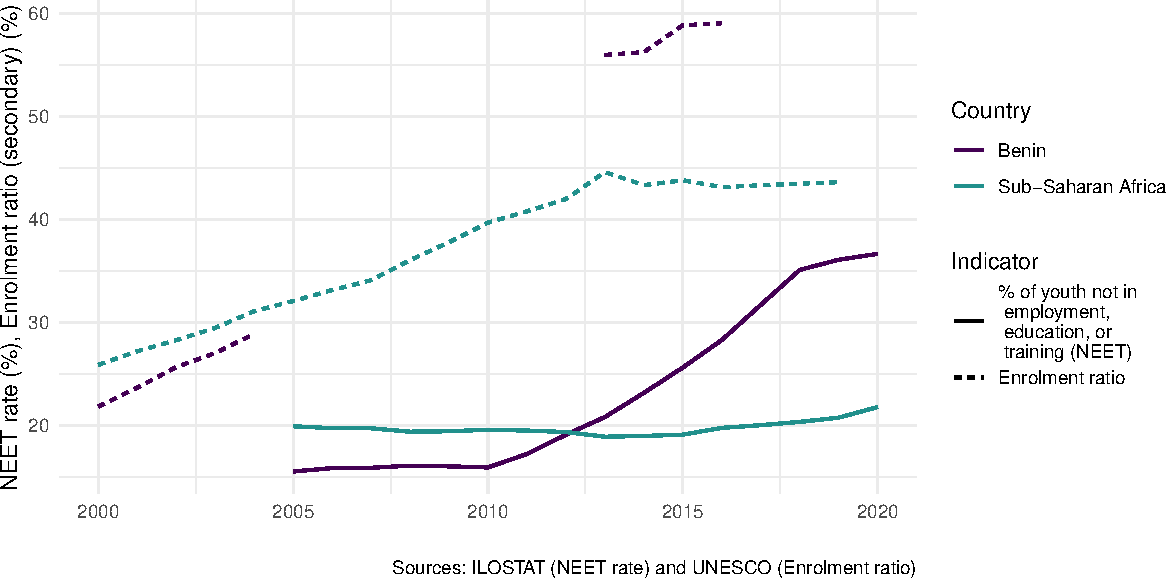
\includegraphics{figures/fig-enrollment-1} \caption{Rates of youth enrollment and inactivity: Bénin and SSA}\label{fig:fig-enrollment}
\end{figure}

As enrollment in formal education has not translated to increasing rates of youth employment, interest in promoting alternative pathways to the labor force has grown. In Bénin, entry into formal technical and vocational education and training (TVET) begins after the completion of the second year of secondary school, or nine years of education. Yet across the country, the median number of years spent in the education system is just four; only five percent of youth of secondary school age are enrolled in TVET (ILO, 2021), in line with the six percent of young workers estimated to participate in formal TVET across SSA (Hofmann et al., 2022). Thus, rather than formal TVET, it is informal apprenticeship that is the primary conduit into the labor market for early school leavers in Bénin, with as many as 300,000 young men and women estimated to be in training (ILO, 2021). Recent examples of investment in Bénin's apprenticeship system include \$6.3 million from the World Bank's for the Benin Youth Employment Project (PEJ), completed in 2019, and a planned \$16.4 million dollar investment in strengthening the TVET system starting in 2020 (World Bank, 2020).

In 2005, the government of Bénin announced a restructuring of traditional apprenticeship in the informal sector. Two national apprenticeship schemes were introduced: a formalization of informal, firm-based apprenticeship called the \emph{Certificat de Qualification aux Métiers}, which introduced a national certificate for the completion of traditional training, and the dual system \emph{Certificat de Qualification Professionnelle} (CQP) program, which sought to combine in-firm, firm-specific training with more general classroom-based teaching, and to accredit the training though a separate nationally-recognized certificate. The three stated objectives of the CQP reform were to (i) offer practical and theoretical training to youth under apprenticeship contracts in the craft sector (ii) train a high-performance labor force; and (iii) improve the productivity and profitability of workshops in the craft sector (Davodoun, 2011).

The CQP is currently available for 13 out of the more than 300 trades listed in the craft sector: auto mechanics, motorcycle mechanics, air conditioning installers, tailors, masons, carpenters, metalworkers (primarily welding of gates for living compounds), electricians, and plumbers (\emph{Swisscontact}, 2019)\footnote{This selection of trades was based at least in part on existing trades from early experimental dual training programs to take advantage of existing training center infrastructure. The CQM is available for about 50 trades.}. To participate in the CQP, applicants must (i) be at least 14 years old, unless otherwise authorized by the labor inspector; (ii) have a written apprenticeship contract that complies with labor laws; (iii) have completed at least 6 years of formal schooling; and (iv) pass a national entry examination (\emph{{KOF}}, 2017). Firm owners apply on behalf of the apprentices already in their charge, generally through local craftsmen associations. After three to four years of training, CQP apprentices may attempt the final examination, which takes place on one date a year for the entire nation, has a practical and a written component, and is overseen by state representatives and local craftsmen. Upon successful completion, apprentices receive a nationally-recognized certificate and have the option to pursue further technical and professional studies if they so desire.

The main government organs tasked with the administration of the CQP are the national TVET directorate (DETFP), which is in charge of apprentice recruitment and training center accreditation, the Direction of Test and Exam Services (DEC), in charge of the entrance and exit examinations, and FODEFCA, responsible for procuring and distributing funding for the program (Nouatin et al., 2019). The CQP began curriculum planning in 2005 with technical assistance from the French Development Agency (AFD) and the Swiss Agency for Development and Cooperation (SDC), among others, and became operational in 2008. In 2012, management of the program passed from Swisscontact, a Swiss NGO, entirely into the hands of FODEFCA (Nouatin et al., 2019). Cost sharing for the CQP program is shared by the state and the apprentice, with the state financing body for dual apprenticeship, FODEFCA, officially taking on 90 percent of the training costs (\emph{{KOF}}, 2017). However, FODEFCA is largely reliant on external donor funding, and regular financing has been an issue for the program in recent years (David-Gnahoui and Ahouangnivo, 2017). The financing of dual training comprises three main budget items: the costs of training to the firm, the administration of the vocational training center, and expenses for entry tests, the final examination, and certification. While on-the-job training in the firm is paid for by the apprentice or their parents, activities in the vocational training centers are largely financed through FODEFCA from various sources (national budget, donors, NGOs, etc.). Certification upon successful completion of the CQP is allocated to the national budget via the Directorate of Examinations, DEC (David-Gnahoui and Ahouangnivo, 2017).

\hypertarget{sampling-and-attrition}{%
\subsection{Sampling and Attrition}\label{sampling-and-attrition}}

The data for this study was collected in two separate surveys. The first consisted of interviews with apprentices who had applied to the 2019 cohort of the CQP program; the second was conducted with the firm owners, or master craftsmen, of their respective training firms. To allow for trade-level controls and to reduce travel distances for interviews, apprentices were randomly selected from a subsample of all CQP applicants: those training in electrical installation, carpentry, masonry, metalwork or plumbing workshops in the southernmost regions of Bénin.

\begin{longtable}[]{@{}
  >{\raggedright\arraybackslash}p{(\columnwidth - 6\tabcolsep) * \real{0.25}}
  >{\raggedright\arraybackslash}p{(\columnwidth - 6\tabcolsep) * \real{0.25}}
  >{\raggedright\arraybackslash}p{(\columnwidth - 6\tabcolsep) * \real{0.25}}
  >{\raggedright\arraybackslash}p{(\columnwidth - 6\tabcolsep) * \real{0.25}}@{}}
\caption{\label{tab:sampling} Apprentice Sampling}\tabularnewline
\toprule
CQP Status & Explanation & Apprentice Survey & Firm Survey \\
\midrule
\endfirsthead
\toprule
CQP Status & Explanation & Apprentice Survey & Firm Survey \\
\midrule
\endhead
Selected & Applied to CQP in 2019 through master craftsmen. Passed exam and was selected. & Random sampling from list of all CQP applicants in five chosen trades and from southern Bénin) & MC assesses \emph{at most} two apprentices, randomly chosen from all CQP selected/not selected in firm at baseline. \\
& & & \\
Not selected & Applied to CQP in 2019 through master craftsmen. Was not selected due to exam score or lack of proximate training center. & Random sampling from list of all CQP applicants in five chosen trades and from southern Bénin) & MC assesses \emph{at most} two apprentices, randomly chosen from all CQP selected/not selected in firm at baseline. \\
& & & \\
Did not apply & Did not apply to CQP. Training as traditional apprentice. & N/A & MC lists \emph{up to} 5 apprentices who did not apply to CQP. Assesses only one, randomly chosen at baseline. \\
\bottomrule
\end{longtable}

\noindent In addition to questions regarding training practices and firm performance, master craftsmen were asked to assess specific apprentices training at their firm. Up to two CQP applicants per firm\footnote{Only CQP applicants who had participated in the apprentice survey could be assessed individually by MCs.} were selected for this exercise. In addition, a single apprentice who had not applied to the CQP was assessed by the craftsman in a similar manner, if there was such an apprentice training in the firm\footnote{As the apprentice survey consisted only of applicants to the program, the only data on non-applicants comes from master craftsmen.}. The sampling procedure for choosing the apprentices for these personal assessments is summarized in Table \ref{tab:sampling} above.

The baseline wave for the two surveys was collected in July-August 2019. The apprentice survey included questions on training characteristics, employment outcomes, their own skills and competences, and the perceived quality of their training, while the firm survey included questions on worker characteristics, wages, and firm expenses and revenues. We additionally surveyed all MCs about the firm's training practices and expenses, as well as their perception of up to three individual apprentices' skills, experience, diligence, efficiency, learning ability, and so on (sampling procedure detailed above). Data on 427 apprentices working for 197 unique firms was collected at baseline. Descriptive statistics for apprentices and firms are shown in Table \ref{tab:tbl-desc} below.

\begin{table}[H]

\caption{\label{tab:tbl-desc}Descriptive Statistics}
\centering
\begin{threeparttable}
\resizebox{\linewidth}{!}{
\begin{tabular}[t]{lccccc}
\toprule
\multicolumn{1}{c}{ } & \multicolumn{2}{c}{Overall} & \multicolumn{3}{c}{By baseline status} \\
\cmidrule(l{3pt}r{3pt}){2-3} \cmidrule(l{3pt}r{3pt}){4-6}
\textbf{Characteristic} & \textbf{Baseline} & \textbf{Endline} & \textbf{Selected} & \textbf{Not Selected} & \textbf{Did Not Apply}\\
\midrule
\addlinespace[0.3em]
\multicolumn{6}{l}{\textbf{Apprentices}}\\
\hspace{1em}N & 427 & 240 & 149 & 107 & 171\\
\hspace{1em}Age & 21.3 (3.4) & 23.2 (3.5) & 21.7 (2.8) & 22.3 (4.1) & 20.1 (3.2)\\
\hspace{1em}Male & 98\% & 98\% & 99\% & 98\% & 97\%\\
\hspace{1em}Trade &  &  &  &  \vphantom{1} & \\
\hspace{1em}\hspace{1em}Masonry & 21\% & 18\% & 19\% & 23\% & 22\%\\
\hspace{1em}\hspace{1em}Carpentry & 11\% & 11\% & 13\% & 6.5\% & 12\%\\
\hspace{1em}\hspace{1em}Plumbing & 13\% & 15\% & 17\% & 11\% & 9.4\%\\
\hspace{1em}\hspace{1em}Metalworking & 20\% & 20\% & 28\% & 12\% & 19\%\\
\hspace{1em}\hspace{1em}Electrical Inst. & 35\% & 36\% & 22\% & 47\% & 38\%\\
\hspace{1em}Years in training & 2.33 (1.38) & 4.39 (1.38) & 2.52 (1.24) & 2.64 (1.30) & 1.92 (1.48)\\
\hspace{1em}Status at endline &  &  &  &  & \\
\hspace{1em}\hspace{1em}Still training & - & 73\% & 92\% & 69\% & 55\%\\
\hspace{1em}\hspace{1em}Graduated & - & 17\% & 6.7\% & 29\% & 21\%\\
\hspace{1em}\hspace{1em}Dropped out & - & 2.5\% & 1.1\% & 1.7\% & 3.6\%\\
\hspace{1em}\hspace{1em}Unknown & - & 7.1\% & 0\% & 0\% & 20\%\\
\hspace{1em}Education &  &  &  &  & \\
\hspace{1em}\hspace{1em}None & 2.5\% & 3.3\% & 0\% & 0.9\% & 6.0\%\\
\hspace{1em}\hspace{1em}<Primary & 15\% & 15\% & 6.0\% & 6.5\% & 30\%\\
\hspace{1em}\hspace{1em}Primary & 22\% & 21\% & 21\% & 32\% & 17\%\\
\hspace{1em}\hspace{1em}Secondary & 57\% & 57\% & 66\% & 59\% & 45\%\\
\hspace{1em}\hspace{1em}Technical & 2.0\% & 2.5\% & 2.7\% & 0.9\% & 2.0\%\\
\hspace{1em}\hspace{1em}Tertiary & 1.5\% & 1.3\% & 3.4\% & 0.9\% & 0\%\\
\addlinespace[0.3em]
\hline
\multicolumn{6}{l}{\textbf{Firms}}\\
\hspace{1em}N & 197 & 150 &  &  & \\
\addlinespace[0.3em]
\multicolumn{6}{l}{\hspace{1em}Apprentices trained}\\
\hspace{1em}\hspace{1em}Total & 5.4 (4.7) & 5.5 (6.0) &  &  & \\
\hspace{1em}\hspace{1em}Selected & 1.20 (1.82) & 1.10 (1.55) &  &  & \\
\hspace{1em}\hspace{1em}Not Selected & 1.47 (2.68) & 1.41 (2.86) &  &  & \\
\hspace{1em}\hspace{1em}Did Not Apply & 2.7 (3.1) & 2.8 (3.1) &  &  & \\
\addlinespace[0.3em]
\multicolumn{6}{l}{\hspace{1em}Firm size}\\
\hspace{1em}\hspace{1em}Total (calculated)¹ & 8.8 (9.1) & 8.2 (8.6) &  &  & \\
\hspace{1em}\hspace{1em}Total (reported) & 6.7 (7.5) & 6.6 (7.1) &  &  & \\
\hspace{1em}\hspace{1em}Apprentices & 5.4 (4.7) & 5.5 (6.0) &  &  & \\
\hspace{1em}\hspace{1em}Permanent wage & 0.36 (1.8) & 0.80 (2.8) &  &  & \\
\hspace{1em}\hspace{1em}Paid family & 0.06 (0.4) & 0.14 (0.6) &  &  & \\
\hspace{1em}\hspace{1em}Unpaid family & 0.05 (0.4) & 0.03 (0.2) &  &  & \\
\hspace{1em}\hspace{1em}Occasional & 0.83 (2.6) & 0.83 (2.3) &  &  & \\
\hspace{1em}Trade &  &  &  &  & \\
\hspace{1em}\hspace{1em}Masonry & 23\% & 20\% &  &  & \\
\hspace{1em}\hspace{1em}Carpentry & 12\% & 12\% &  &  & \\
\hspace{1em}\hspace{1em}Plumbing & 13\% & 14\% &  &  & \\
\hspace{1em}\hspace{1em}Metalworking & 20\% & 21\% &  &  & \\
\hspace{1em}\hspace{1em}Electrical Inst. & 32\% & 33\% &  &  & \\
\bottomrule
\end{tabular}}
\begin{tablenotes}
\small
\item N; Mean (SD); %
\item[1] Calculated by author by summing number of partners, permanent employees, paid and unpaid family workers, occasional workers, and apprentices reported to be working for MC (total firm size reported separately).
\end{tablenotes}
\end{threeparttable}
\end{table}

\noindent Summary statistics from the baseline survey show the sample to be predominantly male youth who, though of average age for an apprenticeship at 21.3 years (ILO, 2022), are significantly more educated than is typical for traditional apprentices, with over half having completed at least some secondary schooling. Successful applicants to the CQP have higher education attainment than unsuccessful applicants; all applicants have higher attainment than non-applicants. Applicants also have more experience coming into the CQP than the required six months, with the average applicant having trained for 1.93 years at the time of application. Non-applicants are younger, less educated, and less experienced than applicants at baseline, suggesting that master craftsmen send their most able and veteran apprentices to stand for the dual training entrance exam. This may indicate that the CQP is perceived by MCs as something more akin to a continuing education rather than an entry-level apprenticeship program.

The majority of training firms are small workshops comprising the firm owner --- the master trainer --- and several apprentices. Two firm sizes are shown in Table \ref{tab:tbl-desc}: those stated directly by the firm owner in response to the question, ``How many people (including you and your apprentices) are currently working in your business?'' and those calculated by the author by summing the number of apprentices, partners, paid and unpaid family workers, and occasional workers reportedly participating in firm activities. Using self-reported size, 94.81\% of firms employed a total of five people or less (including the owner) at baseline and 96.79\% of firms employed no more than ten (97.18\% and 99.53\%, respectively, using author-calculated size). Thus, training firms in the sample are small, in line with observations from the informal sector in Ghana (Frazer, 2006; Velenchik, 1995), but also roughly similar to the size distribution of a sample of Swiss firms reported by Mühlemann et al. (2007)\footnote{Our sample has a higher density of firms with three to nine employees, whereas the Swiss sample (which includes non-training firms) has a higher density of firms with three total employees or fewer. This shift can be explained by the large number of apprentices in the Béninese training firm sample: at baseline, the average firm employed about four apprentices for every other type of employee, or a total of 6 apprentices.}.

The endline survey was conducted in August-September 2021. Overall apprentice attrition in our sample, at 43.8\%, is clearly very high, even when compared to studies in similar contexts: for instance, Crépon and Premand (2019) and Hardy et al. (2019) both report youth attrition of around 10\%, though it is generally common for studies of training programs to be affected by high rates of attrition (McKenzie, 2017). Both youth non-response and firm non-response\footnote{Data on apprentices who had not applied to the CQP was only obtained from firm owners, and is thus only subject to firm attrition.} drive attrition in our sample. We assess the severity of this problem by testing for differences between retained and attritted apprentices in terms of relevant baseline characteristics such as CQP participation, trade, or socioeconomic variables. Tables \ref{tab:tbl-attritionapps} in the Appendix gives no indication of such differences. In Table \ref{tab:tbl-attritionappsreg}, also in the Appendix, we estimate a logit model where attrition is a function of CQP status at baseline and other apprentice characteristics; again, we find no systematic bias. At only 1 percent, reported program dropout among CQP participants retained in the sample is very low compared to similar studies, e.g. Crépon and Premand (2019) who report 31.2\% dropout for dual apprenticeships and 32.5\% for traditional apprenticeships. Sample attrition may well be correlated with program dropout, though we are unable to test this with the available data. Finally, despite starting with comparable experience at baseline, unsuccessful applicants to the CQP were much more likely to have graduated after three years than CQP participants --- Covid-19 related interruptions to training and the single annual CQP examination date both likely contributed to the low CQP graduation rate after three years.

Similarly, of 197 firms interviewed at baseline, only 150 could be contacted at endline, for an overall firm attrition rate of 23.9\%. Tables \ref{tab:tbl-attritionfirms} and \ref{tab:tbl-attritionfirmsreg} in the Appendix likewise suggest that firm attrition was not correlated with key firm characteristics such as size or profitability, though a logit model of attrition shows that firms with a higher proportion of CQP participants among their apprentices are somewhat more likely to exit the sample.

\hypertarget{appmethod}{%
\subsection{Estimating Apprentice Benefits}\label{appmethod}}

We first examine the benefits accruing to apprentices over the observed time period of three years. These benefits can be separated into two categories: human capital gains and material benefits.

Human capital gains are measured using a set of trade-specific scores measured separately for each apprentice at baseline and endline. These amount to a simplified version of the ``task approach'' utilized in the technological change literature (Crépon and Premand, 2019; see Dicarlo et al., 2016). Unlike the general tasks used to measure skills in the task approach, however, we measure apprentice knowledge by means of a short test based on CQP curricula. Each question was a multiple choice question, and between 4 and 5 knowledge questions were posed to each apprentice; because apprentices who did not apply to the CQP were not interviewed directly, the knowledge score was only measured for CQP applicants. The questions are reproduced in Appendix \ref{knowqs}.

Our measures of competence and experience, on the other hand, are based on a short roster of tasks drafted in collaboration with local craft experts and practitioners, an approach similar to that employed by Hardy et al. (2019) (all tasks are shown in Appendix \ref{hcqs}). Firms were asked to assess apprentices on this series of 10 to 15 trade-relevant tasks\footnote{Apprentices were asked to self-evaluate their competence at endline using the same metric. Self-evaluation was not initially planned and thus unavailable at baseline}, and the percentage of tasks in which apprentices are deemed competent or experienced (on a binary sclae) constitute their score in each of the two measures. Similar to the task approach, this method allows for worker-level measurement of ability and experience based on tasks performed. Each apprentice received a score in each of the three dimensions.

Regression analysis is then used to examine the impact of dual training on these three measures of apprentice learning. We use the specification

\[ y_{it} = a+\sum_{j}\text{status}_{ij}+\sum_{k}\text{status}_{ik}\text{×}Endline_t+{Endline}_t+\mathbf{X}_{it}+\mathbf{Z}_{jt}+u_{it} \]
where \(y_{it}\) is the outcome for apprentice \(i\) at time \(t\), \(\text{status}_{ij}\) corresponds to apprentice status \(j\) of apprentice \(i\) in the context of the CQP program: either successful applicant, unsuccessful applicant, or non-applicant, and \(\sum_{k}\text{status}_{ik}\text{×}Endline_t+{Endline}_t\) are the interaction of a CQP participation dummy and survey wave and a dummy for CQP non-applicants and survey wave. These interactions identify any gains in learning outcomes that can be linked to CQP participation. \(\mathbf{X}_{it}\) is a column vector of apprentice characteristics, \(\mathbf{Z}_{jt}\) is a column vector of training-related firm characteristics, \(a\) is a constant, and \(u_{it}\) is an error term.

Finally, we assess the material benefits of training accruing to the apprentice, calculated simply as total fees paid less allowances received. These two categories of transactions between MC and apprentices are described in greater detail in the next section.

\hypertarget{firmmethod}{%
\subsection{Estimating Firm Benefits}\label{firmmethod}}

\begin{table}[H]
\caption{Components of net benefit accounting}
\label{tab:cbmodels}
\setlength{\tabcolsep}{8pt}
\renewcommand{\arraystretch}{1.25}
\resizebox{\textwidth}{!}{%
  \begin{tabular}{llllllll}
  \multicolumn{3}{l|}{}                                                              & \multicolumn{5}{c}{\textbf{Model}}                                 \\
  & \textbf{Estimate} & \multicolumn{1}{l|}{\textbf{Assumptions}}        & \textbf{I} & \textbf{II} & \textbf{III} & \textbf{IV} & \textbf{V} \\ \hline
  \multicolumn{8}{l}{\textbf{Benefits}}                                                                                                                   \\ \hline
  Annual fees & Total fees / 4    & \multicolumn{1}{l|}{Four year training duration} & \textbf{\times} & \textbf{\times}  & \textbf{\times}   & \textbf{\times}  & \textbf{\times} \\ \hline
  \begin{tabular}[c]{@{}l@{}}Annual\\ apprentice\\ productivity\end{tabular} &
    \begin{tabular}[c]{@{}l@{}}Average of monthly wages\\ of experienced and \\ inexperienced employee \times \\ \# of months/year operational\end{tabular} &
  \multicolumn{1}{l|}{\begin{tabular}[c]{@{}l@{}}Wages equal to productivity.\\ Apprentice prod. equal to \\ that of untrained employees \\ for first two years and trained \\ employee for final two years\end{tabular}} &
    \textbf{} &
    \textbf{} &
    \textbf{\times} &
    \textbf{\times} &
    \textbf{\times} \\ \hline
  \multicolumn{8}{l}{\textbf{Costs}}                                                                                                                      \\ \hline
  \begin{tabular}[c]{@{}l@{}}Annual\\ allowances\end{tabular} &
    \begin{tabular}[c]{@{}l@{}}Daily allowances \times \, 20 days \times\\ \# of months/year operational\end{tabular} &
  \multicolumn{1}{l|}{\begin{tabular}[c]{@{}l@{}}Apprentices work 20\\ days/month\end{tabular}} &
    \textbf{\times} &
    \textbf{\times} &
    \textbf{\times} &
    \textbf{\times} &
    \textbf{\times} \\ \hline
  \begin{tabular}[c]{@{}l@{}}Annual\\ training\\ expenses\end{tabular} &
    \begin{tabular}[c]{@{}l@{}}Total monthly training \\ expenses / \# of apprentices \times\\ \# of months/year operational\end{tabular} &
  \multicolumn{1}{l|}{\begin{tabular}[c]{@{}l@{}}All reported training\\ expenses are recurring\end{tabular}} &
    \textbf{} &
    \textbf{\times} &
    \textbf{} &
    \textbf{\times} &
    \textbf{\times} \\ \hline
  \begin{tabular}[c]{@{}l@{}}Annual lost\\ trainer\\ productivity\end{tabular} &
    \begin{tabular}[c]{@{}l@{}}Monthly wages of experienced\\ employee \times \, estimated hours of\\ training per month \times\\ \# of trainers/apprentice \times \\ \# of months/year operational\end{tabular} &
  \multicolumn{1}{l|}{\begin{tabular}[c]{@{}l@{}}Wages equal to productivity.\\ All trainers in firm stop\\ working simultaneously\\ when firm pauses activities \\ to train apprentices.\end{tabular}} &
    &
    &
    &
    &
    \textbf{\times}
  \end{tabular}%
}
\end{table}

Firm benefits were calculated using the accounting approach (Gambin et al., 2013; Mühlemann and Wolter, 2014), which relies on survey data from training firms to identify and quantify the costs and benefits arising from training provision. It has only recently started being applied in lower-middle income countries (Bolli et al., 2020; Bolli et al., 2021; Renold et al., 2018). The accounting approach subtracts the costs of training from its benefits and is a simple way of estimating the value that training apprentices generates for the training firm. In a second step, we use regression analysis to assess the impact of hiring additional apprentices, both traditional and CQP dual trainees, on firm outcomes.

The components of the accounting approach used in this study are summarized in Table \ref{tab:tbl-cbmodels}. Firms receive two primary benefits from training apprentices: apprenticeship fees and the apprentices' productive contributions to the firm. Training fees can be paid in full before the commencement of training or split into payment at the beginning, during, and at the conclusion of training (Velenchik, 1995). Five categories of fees were reported by both apprentices and MCs: entry fees, formation (or general training) fees, liberation (or graduation) fees paid at the conclusion of training, fees as compensation for the materials and equipment used in training, contract fees, and application fees\footnote{Fees are often paid in kind rather than in cash.}. Fees were reported as the total paid for the entirety of the apprenticeship; we assume four-year apprenticeships to estimate annual ammounts.

The second benefit of training for firms, apprentices' net productive contributions, were not reported explicitly by the firm owners and thus needed to be estimated with the aid of several assumptions. First, we assume the competitive model of labor markets (with heterogeneous wages), in which workers are paid the marginal product of their labor. Second, we assume apprentice productivity is equal to that of an untrained employee with no more than a primary education for the first two years of training, and increases to that of trained employee for the final two years\footnote{This is a simplification of the approach used by @bolli2020, in which apprentice productivity is estimated to increase linearly from that of an unskilled worker to that of a skilled worker between defined points in their training. A popular alternative to this approach involves eliciting specific tasks performed by apprentices and estimating costs savings based on the wages paid to workers who would otherwise be responsible for said tasks [@hauschildt2018]. Our firm-apprentice data did not cover specific tasks and is thus not equipped to carry out such an analysis.}, and we use detailed wage information reported by firm owners to estimate the average annual productivity over the course of a four-year apprenticeship. Under these assumptions, the annual productive value generated by apprentice work amounts to the average of these two wages.

Costs of apprenticeship for the firm are categorized into three categories: allowances, training expenses, and lost trainer productivity. Allowances are disbursed irregularly by the firm owner for small expenses such as travel and meals. These are reported by firms at the apprentice level (separate reported allowances for each apprentice). To estimate total annual allowance expenditures per apprentice, we thus sum over all allowance categories and assume that apprentices work 20 days per month; the extrapolated monthly sum is then multiplied by the number of months the training firm was operating in the past year to arrive at an annual estimate for each apprentice. Alternative estimates using different workload assumptions or substituting firm-reported with apprentice-reported figures are shown in Table \ref{tab:tbl-allowancebounds} and Table \ref{tab:tbl-allowboundsapp} in the Appendix.

To help estimate the training costs paid by the firm, owners were asked to identify any costs directly or indirectly related to their training activities. Specific training costs include equipment costs, which comprise all costs for physical infrastructure necessary for training; raw materials such as cement, lumber, or scrap metal used for demonstration or practice purposes; training equipment such as workbenches, toolkits, or other machines purchased or rented specifically for apprentices; rent for training facilities if training was not conducted exclusively in the MC's workshop; and books and any other training materials. Firms reported the training costs in each category for the month prior to the interview; to estimate annual training costs per apprentice per year, the reported firm-level costs are divided by the number of apprentices training in the firm and multiplied by the number of months the firm was open in the previous year.

An additional cost paid by the training firm comes in the form of time lost by training staff when they would have otherwise been engaged in productive activities. Lost trainer productivity is, like apprentice productivity, estimated using wage data. Hourly wages for skilled employees were calculated from monthly wage data and multiplied by the number of hours that the workshop stopped all productive activities to train apprentices in the previous week, as reported by MC. This estimate is burdened by the largest number of assumptions: it is uncertain whether all employees who train apprentices in the firm (a number reported by the MC) stop work entirely while the workshop takes a break to train; whether the majority of lost productivity occurs during these breaks, or in the otherwise normal operation of the firm during which they must also tend to the apprentices. Moreover, the total duration of these breaks in the past week is a very small sample from which to extrapolate to annual costs. Lacking a better method, we report these estimates as the final cost component.

Net benefits were calculated by subtracting some or all of the costs listed above from some or all of the benefits. The simplest model, Model I in \ref{tab:tbl-cbmodels} above, reduces the value of training accruing to the firm to the direct material incomes and expenditures from training; namely, apprenticeship fees from the apprentices and their parents, an approximation of training costs, and the total reported allowances disbursed to the apprentice. Models II and III add training expenses and estimated apprentice productivity, respectively, while Model IV combines all four components. Model V includes all costs and benefits, including lost trainer productivity.

In a final step, we study the effect of hiring apprentices, both traditional and those participating in the CQP, on firm size and profits by estimating the following regression:

\[ y_{it} =  a+CQP_i+{Endline}_t+apprentices_{it}+\mathbf{X}_{it}+u_{it}, \]

where \(y_{it}\) is the outcome of interest, \(CQP_i\) is the number of CQP applicants who were accepted into the 2019 cohort of the program. \(apprentices_{it}\) controls for the total number of apprentices training with the firm and not participating in the CQP program (and in contrast to \(CQP_i\) is a time-varying measure), while \(\mathbf{X}_{it}\) is a matrix of additional covariates for firm \(i\) in wave \(t\), \({Endline}_t\) is a dummy variable denoting survey wave, \(a\) is a constant, and \(u_{it}\) is an error term.

\FloatBarrier

\hypertarget{results}{%
\section{Results}\label{results}}

\hypertarget{appbenefits}{%
\subsection{Impact of Informal and Dual Training on Individuals}\label{appbenefits}}

\begin{table}[H]

\caption{\label{tab:tbl-skills}Change in apprentice human capital}
\centering
\resizebox{\linewidth}{!}{
\begin{threeparttable}
\begin{tabular}[t]{lcccccc}
\toprule
 & \textbf{N} & \textbf{Baseline} & \textbf{N} & \textbf{Endline} & \textbf{Difference} & \textbf{p-value³}\\
\midrule
\addlinespace[0.3em]
\multicolumn{7}{l}{\textbf{Competence¹}}\\
\hspace{1em}Electrical Installation & 125 & 0.80 (0.24) & 69 & 0.96 (0.09) & 0.09 & <0.001\\
\hspace{1em}Masonry & 90 & 0.75 (0.22) & 39 & 0.90 (0.18) & 0.14 & 0.008\\
\hspace{1em}Carpentry & 48 & 0.76 (0.28) & 21 & 0.93 (0.15) & 0.12 & 0.14\\
\hspace{1em}Plumbing & 54 & 0.73 (0.29) & 26 & 0.92 (0.15) & 0.15 & 0.008\\
\hspace{1em}Metalwork & 86 & 0.75 (0.22) & 38 & 0.86 (0.21) & 0.09 & 0.006\\
\hspace{1em}CQP Selected & 143 & 0.81 (0.21) & 82 & 0.95 (0.11) & 0.11 & <0.001\\
\hspace{1em}CQP Not Selected & 95 & 0.84 (0.19) & 56 & 0.94 (0.10) & 0.06 & 0.017\\
\hspace{1em}Did Not Apply & 165 & 0.68 (0.28) & 55 & 0.84 (0.22) & 0.16 & <0.001\\
\textbf{\hspace{1em}Overall} & \textbf{403} & \textbf{0.76 (0.24)} & \textbf{193} & \textbf{0.92 (0.16)} & \textbf{0.11} & \textbf{<0.001}\\
\addlinespace[0.3em]
\multicolumn{7}{l}{\textbf{Experience¹}}\\
\hspace{1em}Electrical Installation & 125 & 0.77 (0.26) & 69 & 0.96 (0.08) & 0.11 & <0.001\\
\hspace{1em}Masonry & 90 & 0.72 (0.23) & 39 & 0.91 (0.13) & 0.20 & <0.001\\
\hspace{1em}Carpentry & 48 & 0.73 (0.31) & 21 & 0.98 (0.06) & 0.19 & 0.013\\
\hspace{1em}Plumbing & 54 & 0.66 (0.30) & 26 & 0.89 (0.17) & 0.21 & 0.001\\
\hspace{1em}Metalwork & 86 & 0.72 (0.24) & 38 & 0.85 (0.15) & 0.13 & 0.004\\
\hspace{1em}CQP Selected & 143 & 0.78 (0.24) & 82 & 0.93 (0.11) & 0.15 & <0.001\\
\hspace{1em}CQP Not Selected & 95 & 0.80 (0.21) & 56 & 0.94 (0.11) & 0.10 & 0.001\\
\hspace{1em}Did Not Apply & 165 & 0.65 (0.29) & 55 & 0.87 (0.16) & 0.21 & <0.001\\
\textbf{\hspace{1em}Overall} & \textbf{403} & \textbf{0.73 (0.26)} & \textbf{193} & \textbf{0.92 (0.13)} & \textbf{0.15} & \textbf{<0.001}\\
\addlinespace[0.3em]
\multicolumn{7}{l}{\textbf{Knowledge²}}\\
\hspace{1em}Electrical Installation & 77 & 0.90 (0.16) & 49 & 0.93 (0.10) & 0.01 & 0.4\\
\hspace{1em}Masonry & 56 & 0.76 (0.19) & 30 & 0.83 (0.20) & 0.01 & 0.8\\
\hspace{1em}Carpentry & 25 & 0.91 (0.18) & 15 & 0.97 (0.09) & 0.05 & 0.3\\
\hspace{1em}Plumbing & 38 & 0.52 (0.12) & 26 & 0.64 (0.16) & 0.11 & 0.013\\
\hspace{1em}Metalwork & 209 & 0.85 (0.18) & 117 & 0.88 (0.15) & 0.00 & 0.8\\
\hspace{1em}CQP Selected & 144 & 0.75 (0.20) & 84 & 0.80 (0.18) & 0.03 & 0.10\\
\hspace{1em}CQP Not Selected & 103 & 0.79 (0.22) & 59 & 0.84 (0.19) & 0.02 & 0.5\\
\textbf{\hspace{1em}Overall} & \textbf{247} & \textbf{0.77 (0.21)} & \textbf{143} & \textbf{0.81 (0.19)} & \textbf{0.03} & \textbf{0.078}\\
\bottomrule
\end{tabular}
\begin{tablenotes}
\small
\item Mean (SD).
\item[1] Percent of trade-specific tasks apprentice is deemed competent in (competence) or has already successfully attempted (experience), as reported by MC. Total of 10-15 tasks, depending on trade.
\item[2] Percent of trade-specific knowledge questions answered correctly by apprentice. Total of 4 or 5 questions, depending on trade. Not available for apprentices who did not apply to the CQP, as they were not interviewed personally.
\item[3] Paired t-test
\end{tablenotes}
\end{threeparttable}}
\end{table}

First, we investigate whether dual training was successful in realizing its primary objective --- increasing the human capital stock of apprentices. To do so, we study the changes in the three human capital indices described in Section \ref{appmethod} over the observed training period of three years. The changes in the human capital index scores presented in Table \ref{tab:tbl-skills} indicate that informal apprenticeship training is successful in improving sector-specific human capital of the youth in our sample, both for dual training participants and traditional apprentices: overall competence scores increased by 0.46 SDs, experience scores by 0.58 SDs, and knowledge by 0.13 SDs. Significant improvements in competence and experience are observed for apprentices who participated in, unsuccessfully applied to, and did not apply to the CQP alike, though apprentices who did not apply to the CQP show the largest gains in competence and experience as assessed by their MC. This result is in line with the observation that MCs appear to send youth who are already relatively experienced (and educated) to apply for dual training.

A paired t-test also indicates significant improvements in competence and experience between baseline and endline across all trades (improvement in competence for plumbing apprentices is marginally insignificant at standard significance levels). On the other hand, gains in the knowledge metric are not statistically significant for any single trade except plumbing - hence, the overall increase in knowledge is driven by results from plumbing apprentices alone. As the average knowledge scores at baseline were significantly lower for plumbing apprentices than for apprentices in other trades, this result may indicate a shortcoming in the metric itself, which was composed of only up to five questions which did not seem to pose a major challenge for most apprentices in the other four trades. Improvement in knowledge was marginally significant (p \textless{} 0.10) for CQP participants but not for CQP applicants who were not selected (p \textless{} 0.5).

Although mean human capital accumulation is higher for participating CQP apprentices than non-selected CQP applicants across the three indices, this does not translate into statistically significant differences between the two group (Table \ref{tab:tbl-skillschangebycqp} in the Appendix). Nor do we observe a significant effect of dual training on the competence and experience indices when apprentices who did not apply to the CQP are added to the control group. To check if apprentices agree with their MC's assessments of their ability, a self-assessment was included in the apprentice survey at endline. Table \ref{tab:tbl-compexp2} in the Appendix suggests that the two assessments are in general agreement for both the experience and the competence index (the exception again being limited to the plumbing trade, where MCs were relatively critical in their assessment of apprentices' abilities).

\begin{table}[H] \centering 
  \caption{Effects of training on human capital development} 
  \label{tab:tbl-appreg} 
\scriptsize 
\begin{tabular}{@{\extracolsep{-8pt}}lccccccccc} 
\\[-1.8ex]\hline 
\hline \\[-1.8ex] 
\\[-1.8ex] & \multicolumn{3}{c}{Experience} & \multicolumn{3}{c}{Competence} & \multicolumn{3}{c}{Knowledge} \\ 
\\[-1.8ex] & (1) & (2) & (3) & (4) & (5) & (6) & (7) & (8) & (9)\\ 
\hline \\[-1.8ex] 
 CQP Selected (reference) \\ \\ CQP Not Selected & $-$0.02 & $-$0.01 & $-$0.01 & $-$0.004 & 0.01 & 0.02 & 0.002 & $-$0.01 & $-$0.001 \\ 
  & (0.03) & (0.04) & (0.05) & (0.03) & (0.04) & (0.05) & (0.03) & (0.04) & (0.05) \\ 
  CQP Did Not Apply & $-$0.05 & $-$0.05 & $-$0.06 & $-$0.09$^{***}$ & $-$0.07$^{*}$ & $-$0.08$^{*}$ &  &  &  \\ 
  & (0.03) & (0.04) & (0.04) & (0.03) & (0.04) & (0.04) &  &  &  \\ 
  Endline & 0.21$^{***}$ & 0.19$^{***}$ & 0.18$^{***}$ & 0.14$^{***}$ & 0.13$^{***}$ & 0.11$^{**}$ & 0.06$^{*}$ & 0.08$^{*}$ & 0.05 \\ 
  & (0.03) & (0.05) & (0.05) & (0.03) & (0.05) & (0.05) & (0.03) & (0.05) & (0.04) \\ 
  CQP Selected x Endline &  & 0.02 & 0.03 &  & 0.05 & 0.04 &  & $-$0.04 & $-$0.01 \\ 
  &  & (0.07) & (0.07) &  & (0.07) & (0.08) &  & (0.07) & (0.06) \\ 
  CQP Did Not Apply x Endline &  & 0.03 & 0.10 &  & $-$0.03 & 0.08 &  &  &  \\ 
  &  & (0.07) & (0.08) &  & (0.07) & (0.08) &  &  &  \\ 
  Baseline Experience$^1$ & 0.06$^{***}$ & 0.06$^{***}$ & 0.06$^{***}$ & 0.06$^{***}$ & 0.06$^{***}$ & 0.06$^{***}$ & 0.02 & 0.02 & $-$0.001 \\ 
  & (0.01) & (0.01) & (0.01) & (0.01) & (0.01) & (0.02) & (0.01) & (0.01) & (0.02) \\ 
  Years of Schooling & 0.005 & 0.01 & $-$0.01 & 0.02 & 0.02 & 0.01 & 0.001 & $-$0.0002 & 0.01 \\ 
  & (0.02) & (0.02) & (0.04) & (0.02) & (0.02) & (0.04) & (0.03) & (0.03) & (0.03) \\ 
  Firm Size$^2$ & 0.01$^{***}$ & 0.01$^{***}$ & 0.04 & 0.01$^{***}$ & 0.01$^{***}$ & 0.05 & 0.01$^{***}$ & 0.01$^{***}$ & 0.004 \\ 
  & (0.002) & (0.002) & (0.04) & (0.002) & (0.002) & (0.04) & (0.003) & (0.003) & (0.04) \\ 
  Total Apprentices in Firm & 0.54$^{***}$ & 0.53$^{***}$ & 0.52$^{**}$ & 0.57$^{***}$ & 0.56$^{***}$ & 0.44$^{**}$ & 0.64$^{***}$ & 0.65$^{***}$ & 0.73$^{***}$ \\ 
  & (0.05) & (0.05) & (0.20) & (0.05) & (0.05) & (0.21) & (0.06) & (0.06) & (0.21) \\ 
 \hline \\[-1.8ex] 
Firm FE & NO & NO & YES & NO & NO & YES & NO & NO & YES \\ 
Observations & 228 & 228 & 228 & 228 & 228 & 228 & 148 & 148 & 148 \\ 
R$^{2}$ & 0.35 & 0.35 & 0.77 & 0.32 & 0.32 & 0.73 & 0.08 & 0.09 & 0.89 \\ 
F Statistic & 20.00$^{***}$ & 15.00$^{***}$ & 3.60$^{***}$ & 17.00$^{***}$ & 13.00$^{***}$ & 2.90$^{***}$ & 2.60$^{**}$ & 2.20$^{**}$ & 4.20$^{***}$ \\ 
\hline 
\hline \\[-1.8ex] 
\textit{Note:}  & \multicolumn{9}{r}{$^{*}$p$<$0.1; $^{**}$p$<$0.05; $^{***}$p$<$0.01} \\ 
 & \multicolumn{9}{r}{$^1$Years of training prior to baseline survey} \\ 
 & \multicolumn{9}{r}{$^2$Excluding apprentices.} \\ 
\end{tabular} 
\end{table}

\noindent The estimated effects of training presented in Table \ref{tab:tbl-appreg} confirm that apprentice human capital, as measured by the three indices, increases after three years, and that apprentices who do not apply to the CQP program score somewhat lower on the competence index. Higher baseline experience and competence scores for CQP applicants suggest that trainers send their more able apprentices to apply for dual training. The selection process for the program itself, however, does not favor more experienced apprentices according to our metrics (i.e.~is as good as random).

Participation in the CQP program is shown to have no detectable effect on human capital accumulation; in fact, when controlling for individual effects, we find that apprentices who did not apply to the CQP make larger gains on the competence and experience indices relative to non-selected CQP applicants, while CQP participants do not (columns (3) and (6) in Table \ref{tab:tbl-appreg}). The regression estimates also suggest that apprentice experience and the number of other apprentices training in the firm are correlated with somewhat higher index scores. Table \ref{tab:tbl-appreg2} in the Appendix shows the same regression estimates using a restricted sample of CQP program applicants (successful and unsucessful) only, with the same result: there is no detectable effect of dual training on apprentice experience or competence.

\begin{table}[H]

\caption{\label{tab:tbl-netappbenefits}Annual costs and benefits accruing to apprentice}
\centering
\resizebox{\linewidth}{!}{
\begin{threeparttable}
\begin{tabular}[t]{lccccc}
\toprule
\textbf{Characteristic} & \textbf{Overall} & \textbf{CQP Selected} & \textbf{CQP Not Selected} & \textbf{Did Not Apply} & \textbf{p-value³}\\
\midrule
\addlinespace[0.3em]
\multicolumn{6}{l}{\textbf{Apprentice survey:}}\\
\hspace{1em}Total Fees & 72.02 (47.76) & 70.52 (48.98) & 74.24 (46.09) & - & 0.6\\
\hspace{1em}\hspace{1em}Entry & 4.22 (13.77) & 3.35 (8.35) & 5.52 (19.15) & - & 0.3\\
\hspace{1em}\hspace{1em}Formation & 41.80 (37.40) & 40.32 (35.60) & 43.98 (40.02) & - & 0.5\\
\hspace{1em}\hspace{1em}Liberation & 9.86 (19.87) & 10.00 (19.64) & 9.65 (20.32) & - & >0.9\\
\hspace{1em}\hspace{1em}Materials & 6.97 (8.48) & 7.31 (9.39) & 6.47 (6.94) & - & 0.4\\
\hspace{1em}\hspace{1em}Contract & 6.32 (15.24) & 6.42 (15.67) & 6.17 (14.65) & - & >0.9\\
\hspace{1em}\hspace{1em}Application & 2.85 (3.94) & 3.12 (4.14) & 2.45 (3.61) & - & 0.2\\
\hspace{1em}Allowances¹ & 207.28 (289.76) & 206.68 (319.95) & 208.09 (245.55) & - & >0.9\\
\textbf{\hspace{1em}Allowances net fees²} & \textbf{134.17 (310.94)} & \textbf{141.60 (348.47)} & \textbf{123.60 (249.63)} & \textbf{-} & \textbf{0.7}\\
\addlinespace[0.3em]
\multicolumn{6}{l}{\textbf{Firm survey:}}\\
\hspace{1em}Total Fees & 66.06 (44.54) & 52.53 (36.63) & 56.72 (38.85) & 83.08 (48.31) & <0.001\\
\hspace{1em}\hspace{1em}Entry & 2.74 (4.11) & 2.33 (3.30) & 2.82 (5.29) & 3.03 (3.91) & 0.3\\
\hspace{1em}\hspace{1em}Formation & 35.95 (38.04) & 20.10 (27.58) & 29.04 (33.19) & 53.47 (41.22) & <0.001\\
\hspace{1em}\hspace{1em}Liberation & 9.26 (18.70) & 9.44 (18.61) & 7.26 (17.86) & 10.30 (19.28) & 0.4\\
\hspace{1em}\hspace{1em}Materials & 6.56 (9.31) & 6.35 (9.47) & 6.20 (8.83) & 6.95 (9.49) & 0.8\\
\hspace{1em}\hspace{1em}Contract & 8.46 (16.92) & 11.01 (18.70) & 8.70 (17.52) & 6.18 (14.60) & 0.050\\
\hspace{1em}\hspace{1em}Application & 3.09 (4.24) & 3.30 (4.25) & 2.70 (4.00) & 3.14 (4.38) & 0.6\\
\hspace{1em}Allowances & 278.07 (388.14) & 243.10 (412.21) & 341.82 (458.15) & 272.50 (332.72) & 0.3\\
\hspace{1em}\hspace{1em}Food & 70.57 (147.07) & 61.57 (158.26) & 89.31 (190.63) & 68.07 (113.25) & 0.5\\
\hspace{1em}\hspace{1em}Transport & 60.88 (195.20) & 46.23 (188.52) & 79.61 (227.49) & 62.18 (184.29) & 0.6\\
\hspace{1em}\hspace{1em}Pocket money & 145.96 (183.74) & 135.30 (169.17) & 172.89 (197.68) & 140.85 (186.83) & 0.5\\
\hspace{1em}\hspace{1em}Other & 0.65 (10.64) & 0.00 (0.00) & 0.00 (0.00) & 1.39 (15.52) & 0.6\\
\textbf{\hspace{1em}Allowances net fees²} & \textbf{212.77 (398.58)} & \textbf{199.11 (433.21)} & \textbf{272.12 (472.83)} & \textbf{195.68 (337.65)} & \textbf{0.5}\\
\bottomrule
\end{tabular}
\begin{tablenotes}
\small
\item Mean (SD). Amounts in \$US per apprentice per year, calculated using responses from baseline survey. Annual fees assume apprenticeship duration of four years.
\item[1] Apprentices were only asked about total allowances received.
\item[2] Rows missing all allowance or all fee data were excluded from net benefit calculation. Mean net benefit may deviate from difference in mean allowances and mean fees as a result.
\item[3] Student's t-test for apprentice survey data, analysis of variance for firm survey data
\end{tablenotes}
\end{threeparttable}}
\end{table}

\noindent Table \ref{tab:tbl-netappbenefits} shows estimates of the apprentices' net cost of training, taking into account training fees and allowances as outlined in Section \ref{appmethod}. Overall, apprentices receive more in allowances from their trainer over the course of the training period (assuming a four-year training duration) than they (or their parents) pay in total fees. Mean net benefits amount to about 82000 FCFA (135 \$US) per apprentice per year according to apprentices' own estimates and 128000 FCFA (212 \$US) according to the firm survey.

Formation fees (i.e.~general training fees) constitute the largest transfer from the apprentice to the MC. Apprentices report significantly higher fees than the MC, for the training fee in particular. Firms may underreport fees to avoid accusations of gauging, but are at the same time likely to have more direct knowledge of all fees than apprentices, whose parents and relatives usually pay the craftsmen directly.

We observe no statistically significant differences across CQP status in terms of net benefits or allowances received. Apprentices do not report paying different fees if they participated in the CQP (relative to those that applied but were not selected), whereas MCs report charging lower fees for CQP applicants (selected and not selected) than for traditional apprentices. This may reflect a reporting bias wherein CQP applicants, who were more experienced at baseline, paid their fees at a more distant point in the past, causing MCs to underreport their total value.

\hypertarget{firmimpact}{%
\subsection{Impact of Informal and Dual Training on Firms}\label{firmimpact}}

\begin{table}[H]

\caption{\label{tab:tbl-netbenefits}Annual costs and benefits per apprentice accruing to firm}
\centering
\resizebox{\linewidth}{!}{
\begin{threeparttable}
\begin{tabular}[t]{lcccccc}
\toprule
\textbf{Characteristic} & \textbf{N} & \textbf{Overall} & \textbf{CQP Selected} & \textbf{CQP Not Selected} & \textbf{Did Not Apply} & \textbf{p-value²}\\
\midrule
\addlinespace[0.3em]
\multicolumn{7}{l}{\textbf{Benefits}}\\
\hspace{1em}Fees¹ & 403 & 65.30 (44.66) & 50.74 (36.67) & 57.68 (39.33) & 83.08 (48.31) & <0.001\\
\hspace{1em}\hspace{1em}Entry & 391 & 2.74 (4.11) & 2.33 (3.30) & 2.82 (5.29) & 3.03 (3.91) & 0.3\\
\hspace{1em}\hspace{1em}Formation & 391 & 35.95 (38.04) & 20.10 (27.58) & 29.04 (33.19) & 53.47 (41.22) & <0.001\\
\hspace{1em}\hspace{1em}Liberation & 391 & 9.26 (18.70) & 9.44 (18.61) & 7.26 (17.86) & 10.30 (19.28) & 0.4\\
\hspace{1em}\hspace{1em}Materials & 391 & 6.56 (9.31) & 6.35 (9.47) & 6.20 (8.83) & 6.95 (9.49) & 0.8\\
\hspace{1em}\hspace{1em}Contract & 391 & 8.46 (16.92) & 11.01 (18.70) & 8.70 (17.52) & 6.18 (14.60) & 0.050\\
\hspace{1em}\hspace{1em}Application & 391 & 3.09 (4.24) & 3.30 (4.25) & 2.70 (4.00) & 3.14 (4.38) & 0.6\\
\hspace{1em}Apprentice prod. & 114 & 1,075.59 (1,172.98) & 869.20 (1,050.46) & 1,246.57 (1,294.84) & 1,118.48 (1,183.45) & 0.4\\
\textbf{\hspace{1em}Total} & \textbf{104} & \textbf{1,140.89 (1,198.06)} & \textbf{939.01 (1,059.45)} & \textbf{1,302.16 (1,343.08)} & \textbf{1,195.75 (1,212.34)} & \textbf{0.5}\\
\addlinespace[0.3em]
\multicolumn{7}{l}{\textbf{Costs}}\\
\hspace{1em}Allowances¹ & 360 & 489.37 (1,021.21) & 583.89 (1,398.96) & 632.85 (949.56) & 272.50 (332.72) & 0.012\\
\hspace{1em}\hspace{1em}Food & 266 & 70.57 (147.07) & 61.57 (158.26) & 89.31 (190.63) & 68.07 (113.25) & 0.5\\
\hspace{1em}\hspace{1em}Transport & 266 & 60.88 (195.20) & 46.23 (188.52) & 79.61 (227.49) & 62.18 (184.29) & 0.6\\
\hspace{1em}\hspace{1em}Pocket money & 266 & 145.96 (183.74) & 135.30 (169.17) & 172.89 (197.68) & 140.85 (186.83) & 0.5\\
\hspace{1em}\hspace{1em}Other & 266 & 0.65 (10.64) & 0.00 (0.00) & 0.00 (0.00) & 1.39 (15.52) & 0.6\\
\hspace{1em}Training costs & 229 & 110.69 (233.24) & 110.95 (251.60) & 149.32 (249.61) & 82.63 (196.58) & 0.2\\
\hspace{1em}\hspace{1em}Rent & 229 & 26.83 (59.79) & 24.18 (52.84) & 40.90 (80.34) & 19.55 (47.29) & 0.10\\
\hspace{1em}\hspace{1em}Equipment & 226 & 32.61 (81.94) & 24.75 (50.81) & 56.15 (129.04) & 24.98 (63.74) & 0.046\\
\hspace{1em}\hspace{1em}Books & 224 & 8.93 (44.17) & 7.65 (40.66) & 12.32 (51.90) & 7.96 (42.41) & 0.8\\
\hspace{1em}\hspace{1em}Raw materials & 223 & 44.10 (140.23) & 55.07 (187.93) & 46.60 (107.48) & 30.62 (92.12) & 0.5\\
\hspace{1em}Lost trainer prod. & 245 & 36.08 (45.78) & 37.68 (47.11) & 30.40 (38.00) & 37.97 (48.74) & 0.6\\
\textbf{\hspace{1em}Total} & \textbf{96} & \textbf{666.56 (698.44)} & \textbf{676.45 (673.07)} & \textbf{876.90 (805.36)} & \textbf{464.40 (582.52)} & \textbf{0.082}\\
\addlinespace[0.3em]
\multicolumn{7}{l}{\textbf{Net Benefits}}\\
\hspace{1em}Model I & 341 & -437.12 (1,047.68) & -547.64 (1,422.47) & -588.98 (979.25) & -195.68 (337.65) & 0.008\\
\hspace{1em}Model II & 198 & -480.28 (661.41) & -571.18 (764.74) & -638.96 (670.01) & -237.96 (413.50) & 0.001\\
\hspace{1em}Model III & 75 & 726.77 (1,275.80) & 444.72 (1,169.03) & 811.85 (1,468.62) & 1,005.74 (1,162.53) & 0.3\\
\hspace{1em}Model IV & 31 & 631.55 (1,406.07) & 78.33 (1,264.37) & 1,209.68 (1,683.05) & 588.84 (691.70) & 0.14\\
\hspace{1em}Model V & 28 & 686.67 (1,378.91) & -8.33 (1,298.95) & 1,525.25 (1,460.55) & 580.85 (688.28) & 0.031\\
\bottomrule
\end{tabular}
\begin{tablenotes}
\small
\item Mean (SD). Amounts in \$US per apprentice per year. Calculated using responses from baseline survey, except training costs which were not elicited until endline. Net benefits are not computed for rows with missing data for any categories included in a given model. Mean net benefit estimates may deviate from sums of the relevant categories as a result.
\item[1] Fees and allowances reported by firm owner. Annual fees assume apprenticeship duration of four years, annual allowances assume apprentices work 20 days a month.
\item[2] Analysis of variance
\end{tablenotes}
\end{threeparttable}}
\end{table}

\noindent Next, we study the net benefits from apprenticeship training accruing to firms. We also investigate whether the presence of dual-system apprentices in the firm impacts productivity relative to firms with fewer or no CQP participants.

To first measure benefits in an accounting sense, we use the five ``models'' summarized in Table \ref{tab:tbl-cbmodels} and described in detail in Section \ref{firmmethod}. Table \ref{tab:tbl-netbenefits} above shows the annual costs and benefits estimated per apprentice for each category, along with estimates by apprentice CQP status. Mean net benefits range from -437 \$US to 687 \$US per apprentice per year, depending on the model used. Apprentice allowances and productivity are the decisive factors determining whether training is profitable for a given apprentice; the sign of the mean of each of the net benefit models thus hinges on the inclusion of the productivity variable (not included in Models I and II; included in Models III-V).

Training fees amount to 65.3\$US per apprentice annually, assuming four years of training. Formation fees represent the largest single fee paid to the firms and account for over half of total fees paid. Other minor fees cover the provision of equipment and materials, application fees (pertinent for the CQP, as the master trainer must submit paperwork in their apprentices' stead), and initiation and graduation fees. Firm owners report receiving around 261.21 \$US in total fees per apprentice, or 65.3 per year (assuming 4 years of training). This indicates a minor increase in the costs of training in Bénin over the past two decades: for instance, Walther and Filipiak (2007) reports total fees ranging from 50,000 to 150,000 FCFA (96-290 \$US, inflation adjusted). Apprentices who did not apply to the CQP pay higher training fees and receive less in allowances (both significant at the 2\% level). This also contributes to the significantly lower net costs for this group estimated with Models I and II. Apprentice productivity is calculated using firm-level wage information, an approach similar to apprenticeship cost-benefit studies by Wolter and Mühlemann (2015), Mühlemann et al. (2018), Bolli et al. (2020), and Bolli et al. (2021) and described in Section \ref{appmethod}. The annual productivity estimates reported in Table \ref{tab:tbl-netbenefits} are an order of magnitude higher than the estimated annual benefits from training fees. Because the wage data necessary for estimating apprentice productivity is not available for many of the small firms in the sample, however, apprentice productivity can only be estimated for about a quarter of the sample.

Allowances paid to apprentices by MCs comprise the largest reported cost of training for firms, accounting for 73.42\% of all training costs --- in line with the upper range of costs from David-Gnahoui and Ahouangnivo (2017), who, citing Zinsou, 2012, reported total costs of 100,000 to 250,000 FCFA (\$165-\$413) for a complete CQP training program in 2012. Table \ref{tab:tbl-netbenefits} shows that allowances disbursed to CQP participants and CQP applicants are significantly higher than to non-applicants; as applicants tend to be older and more experienced apprentices, this may suggest that apprentice productivity (or at least their remuneration) tends to increase over time. Expenditures on equipment, raw materials and rent for training spaces, grouped together as non-wage training costs, are the second-largest expenditure for firms and average 110.69\$US, while lost trainer productivity only totals about 36.08\$US --- an order of magnitude less than the estimated expenditure on allowances. These various costs of training per apprentice reported by the MCs are summarized in Figure \ref{fig:fig-costspie} in the Appendix.

The distributions of per-apprentice net benefits have long left tails for Models I and II and long right tails for Models III-V (plotted with their means in Figure \ref{fig:fig-apphist} in the Appendix). The left tails are a consequence of the high number of apprentices in a number of firms generating unrealistic annual allowance totals; these are more than compensated by apprentice productivity estimates when included in Models III-V, skewing the distribution to the right for these models. For models excluding apprentices' productive contributions to the firm (Model I and Model II), we find that apprentices who applied to the CQP program (selected and not selected) are significantly more costly to train (incur higher net costs) on average than non-applicants, on account of the higher allowances MCs report they receive.

Estimates for Models III-V are only available for a small number of apprentices due to the requirement that net benefits only be computed when data for all cost and benefit categories included in the respective model are available. The variance in benefits is high, ranging 4007.02 \$US to net costs of 2005.37 \$US per apprentice per year. Mean net benefits per apprentice per year range from -8.33 \$US to 444.72 \$US for CQP apprentices, 1525.25 \$US to 811.85 \$US for unsuccessful CQP applicants, and 580.85 \$US to 1005.74 \$US for non-applicants. Though large in magnitude, the differences in means between the three groups are not statistically significant for Models III and IV due to the limited sample and high variance. Model V, which includes all cost and benefit categories, generates statistically different estimates for net benefits for the three categories: CQP apprentices are nearly break-even, while unsuccessful CQP applicants generate benefits of -8.33 \$US and non-applicants generate 580.85 \$US. This is only based on a total sample of 28 observations, however.

CQP participants generate significantly lower benefits when unsuccessful CQP applicants only are used as the comparison group according to Models IV and V (\ref{tab:tbl-appnetbenefitsnodna}.

Only 5-11\% of apprentices generate positive net benefits when productivity is left unaccounted for; this rises to about 70\% (at baseline) for Models III-V. According to Model I, 11.14\% and 11.88\% of apprentices are estimated to generate a positive net benefit during training at baseline and endline, respectively; using Model II, 5.05\% and 8.91\% of apprentices are estimated to do so; using Model III, 70.67\% and 66.67\% of apprentices are estimated to do so; using Model IV, 70.97\% and 45.61\% of apprentices are estimated to do so; using Model V, 67.86\% and 42.31\% of apprentices are estimated to do so.

Further tabulations can be found in the Appendix: Table \ref{tab:tbl-appnetbenefitsbywave} shows baseline and endline results, while Table \ref{tab:tbl-appnetbenefitsbytrade} reports cost and benefit estimates by trade.

\begin{table}[H]

\caption{\label{tab:tbl-cblong}Annual net benefits per firm}
\centering
\resizebox{\linewidth}{!}{
\begin{threeparttable}
\begin{tabular}[t]{lccccc}
\toprule
\multicolumn{2}{c}{ } & \multicolumn{4}{c}{\textbf{Firm size¹}} \\
\cmidrule(l{3pt}r{3pt}){3-6}
 & \textbf{Overall}, N = 196 & \textbf{(1,4]}, N = 54 & \textbf{(4,6]}, N = 52 & \textbf{(6,10]}, N = 44 & \textbf{(10,107]}, N = 46\\
\midrule
\addlinespace[0.3em]
\multicolumn{6}{l}{\textbf{Firm Accounts}}\\
\hspace{1em}Revenues & 3,989 (4,820) & 2,059 (1,656) & 2,700 (2,301) & 4,034 (5,233) & 8,028 (6,757)\\
\hspace{1em}Wage bill & 977 (2,357) & 272 (473) & 601 (951) & 783 (994) & 2,446 (4,380)\\
\hspace{1em}Non-wage expenses & 1,600 (3,159) & 810 (734) & 952 (1,298) & 1,473 (2,037) & 3,368 (5,666)\\
\hspace{1em}Total expenses & 2,585 (4,461) & 1,082 (959) & 1,564 (1,777) & 2,256 (2,615) & 5,866 (7,799)\\
\hspace{1em}Profits (reported) & 1,672 (2,634) & 951 (966) & 1,374 (1,247) & 1,567 (1,957) & 3,040 (4,646)\\
\hspace{1em}Profits² (calculated²) & 1,701 (3,056) & 993 (1,390) & 1,393 (1,776) & 1,861 (4,551) & 2,849 (3,518)\\
\addlinespace[0.3em]
\multicolumn{6}{l}{\textbf{Projected benefits}}\\
\hspace{1em}Fees & 349 (366) & 116 (102) & 246 (176) & 374 (249) & 715 (518)\\
\hspace{1em}Apprentice prod. & 8,359 (13,033) & 191 (165) & 1,269 (1,339) & 2,804 (3,099) & 17,280 (16,049)\\
\hspace{1em}Total & 8,887 (13,241) & 363 (255) & 1,334 (1,400) & 3,148 (3,203) & 17,860 (16,023)\\
\addlinespace[0.3em]
\multicolumn{6}{l}{\textbf{Projected costs}}\\
\hspace{1em}Allowances & 3,224 (7,758) & 871 (2,083) & 2,150 (3,544) & 2,681 (4,607) & 7,823 (14,026)\\
\hspace{1em}Training costs & 518 (1,110) & 191 (322) & 385 (539) & 810 (1,887) & 822 (1,191)\\
\hspace{1em}Lost trainer prod. & 181 (421) & 72 (86) & 97 (103) & 136 (190) & 423 (768)\\
\hspace{1em}Total & 3,190 (4,441) & 927 (626) & 2,302 (2,299) & 5,566 (8,254) & 5,546 (3,806)\\
\addlinespace[0.3em]
\multicolumn{6}{l}{\textbf{Net benefits}}\\
\hspace{1em}Model I & -2,963 (7,778) & -774 (2,180) & -1,928 (3,551) & -2,324 (4,536) & -7,187 (14,014)\\
\hspace{1em}Model II & -3,199 (8,563) & -574 (518) & -2,163 (2,403) & -3,267 (5,625) & -8,315 (16,940)\\
\hspace{1em}Model III & 5,574 (12,052) & -571 (792) & -198 (1,142) & 1,134 (4,091) & 11,488 (15,537)\\
\hspace{1em}Model IV & 6,431 (12,457) & -1,039 (757) & -574 (1,290) & 1,225 (6,979) & 11,520 (14,510)\\
\hspace{1em}Model V & 6,593 (12,285) & -1,108 (777) & -617 (1,296) & 4,001 (4,911) & 11,187 (14,678)\\
\bottomrule
\end{tabular}
\begin{tablenotes}
\small
\item Mean (SD). Net benefits per firm estimated using baseline data. 
Projected costs, benefits, and net benefits calculated as mean values for all observed apprentices in 
firm times reported number of apprentices trained. Amounts in \$US.
\item[1] Firms size calculated by author as sum of all reported workers in firm, including apprentices and occasional and family workers.
\item[2] Profits recalculated by author as difference between reported revenues (first row) and reported expenses (second row).
\end{tablenotes}
\end{threeparttable}}
\end{table}

\noindent In a small number of firms, differences in net benefits for individual firms results in apprentices with both positive and negative net benefits to appear in the same firm, resulting in an ambiguous net benefit for the firm. Moreover, we are interested in the importance of apprenticeship training relative to all firm activities, as well as the characteristics of firms hiring high-value apprentices. To address these questions, we estimate firm-level net benefits, calculated as the average costs and benefits of all observed apprentices in a given firm multiplied by the total number of apprentices training at that firm \footnote{As training costs are reported at the firm level and apprentice and trainer productivity estimates were based on firm-reported wage schedules and training frequency, in effect only fee and allowance data is extrapolated in this exercise.}. Firm-level net benefits of training are then calculated using Models I-V from before, and are shown in Table \ref{tab:tbl-cblong} above.

Mean estimated benefits per firm average range from -2409.23 \$US per year to 1254.27 \$US per year, with the large variance in estimates driven once more by apprentice productivity estimates. Table \ref{tab:tbl-cblong} reports estimates by firm size, showing that the largest firms in the sample, through significantly higher reported wages, have significantly higher estimated apprentice productivity.

Allowances are, as in the individual-level estimations, by far the largest cost related to training. Firm-level aggregation suggests that our methodology may in fact overestimate apprentice allowances: for all but the smallest firms, total estimated allowances are on average higher than total firm expenditures reported by the firm.

As with the individual-level estimates, the majority of firms are clustered around zero net benefits for all cost-benefit models, with long left and right tails depending on the model used. Models I and II exhibit long left tails, while Models III-V have long right tails, albeit for fewer observations (plotted with their means in Figure \ref{fig:fig-firmhist} in the Appendix).

According to Model I, 8.89\% and 11.11\% of firms are estimated to earn a positive net benefit from training (positive net benefits) at baseline and endline, respectively; using Model II, 3.33\% are estimated to do so at baseline and 8.89\% at endline, using Model III, 73.08\% are estimated to do so at baseline and 77.27\% at endline; using Model IV, 66.67\% are estimated to do so at baseline and 54.55\% at endline; using Model V, 60\% are estimated to do so at baseline and 53.85\% at endline.

\begin{table}[H] \centering 
  \caption{Firm-level regressions} 
  \label{tab:tbl-firmregs} 
\scriptsize 
\begin{tabular}{@{\extracolsep{-8pt}}lccccccccccc} 
\\[-1.8ex]\hline 
\hline \\[-1.8ex] 
\\[-1.8ex] & \multicolumn{4}{c}{log Revenues} & \multicolumn{4}{c}{log profits} & \multicolumn{3}{c}{log Firm size$^1$} \\ 
\\[-1.8ex] & (1) & (2) & (3) & (4) & (5) & (6) & (7) & (8) & (9) & (10) & (11)\\ 
\hline \\[-1.8ex] 
 No. of Apprentices: \\ \\
                               log CQP Selected & 0.05 & 0.02 & 0.08 & 0.08 & 0.08$^{*}$ & 0.02 & 0.05 & 0.03 & 0.03 & 0.06$^{**}$ & 0.04 \\ 
  & (0.04) & (0.04) & (0.05) & (0.05) & (0.05) & (0.05) & (0.07) & (0.08) & (0.02) & (0.03) & (0.03) \\ 
  log CQP Not Selected/Did Not Apply & 0.29$^{***}$ & 0.24$^{**}$ & 0.23$^{**}$ & 0.28$^{***}$ & 0.23$^{**}$ & 0.20 & 0.20 & 0.23 & 0.05 & 0.05 & 0.03 \\ 
  & (0.08) & (0.09) & (0.09) & (0.10) & (0.10) & (0.13) & (0.13) & (0.15) & (0.06) & (0.06) & (0.06) \\ 
  Endline & 0.33$^{**}$ & 0.41$^{**}$ & 0.56$^{***}$ & 0.49$^{**}$ & $-$0.21 & $-$0.16 & $-$0.10 & $-$0.21 & $-$0.11 & 0.02 & $-$0.05 \\ 
  & (0.13) & (0.16) & (0.18) & (0.21) & (0.16) & (0.22) & (0.25) & (0.31) & (0.11) & (0.12) & (0.13) \\ 
  log Firm Size$^1$ &  & 0.43$^{***}$ & 0.40$^{***}$ & 0.34$^{**}$ &  & 0.42$^{**}$ & 0.41$^{**}$ & 0.50$^{**}$ &  &  &  \\ 
  &  & (0.13) & (0.13) & (0.15) &  & (0.19) & (0.19) & (0.23) &  &  &  \\ 
  log CQP Selected x Endline &  &  & $-$0.12$^{*}$ & $-$0.01 &  &  & $-$0.05 & 0.18 &  & $-$0.10$^{**}$ & $-$0.01 \\ 
  &  &  & (0.07) & (0.12) &  &  & (0.09) & (0.16) &  & (0.05) & (0.07) \\ 
  MC Age &  &  &  & 0.02$^{*}$ &  &  &  & 0.01 &  &  & 0.01 \\ 
  &  &  &  & (0.01) &  &  &  & (0.02) &  &  & (0.01) \\ 
  MC Years of Schooling &  &  &  & 0.01 &  &  &  & 0.01 &  &  & 0.003 \\ 
  &  &  &  & (0.02) &  &  &  & (0.04) &  &  & (0.01) \\ 
  Registered Firm$^2$ &  &  &  & 0.34 &  &  &  & $-$0.14 &  &  & 0.34$^{**}$ \\ 
  &  &  &  & (0.24) &  &  &  & (0.35) &  &  & (0.14) \\ 
  Trade Association &  &  &  & $-$0.32 &  &  &  & $-$0.18 &  &  & 0.21 \\ 
  &  &  &  & (0.26) &  &  &  & (0.38) &  &  & (0.15) \\ 
  Training Frequency$^3$ &  &  &  & $-$0.03 &  &  &  & 0.10 &  &  & $-$0.03 \\ 
  &  &  &  & (0.10) &  &  &  & (0.14) &  &  & (0.05) \\ 
  Constant & 7.40$^{***}$ & 7.30$^{***}$ & 7.30$^{***}$ & 6.80$^{***}$ & 7.00$^{***}$ & 6.90$^{***}$ & 6.80$^{***}$ & 6.10$^{***}$ & 1.30$^{***}$ & 1.20$^{***}$ & 0.94$^{***}$ \\ 
  & (0.13) & (0.23) & (0.23) & (0.56) & (0.17) & (0.33) & (0.34) & (0.96) & (0.10) & (0.10) & (0.33) \\ 
 \hline \\[-1.8ex] 
Trade FE & NO & NO & NO & YES & NO & NO & NO & YES & NO & NO & YES \\ 
Observations & 252 & 112 & 112 & 107 & 200 & 82 & 82 & 78 & 130 & 130 & 124 \\ 
R$^{2}$ & 0.08 & 0.19 & 0.21 & 0.33 & 0.05 & 0.11 & 0.11 & 0.20 & 0.03 & 0.07 & 0.19 \\ 
F Statistic & 7.40$^{***}$ & 6.40$^{***}$ & 5.80$^{***}$ & 3.20$^{***}$ & 3.60$^{**}$ & 2.30$^{*}$ & 1.90 & 1.10 & 1.30 & 2.30$^{*}$ & 1.90$^{**}$ \\ 
\hline 
\hline \\[-1.8ex] 
\textit{Note:}  & \multicolumn{11}{r}{$^{*}$p$<$0.1; $^{**}$p$<$0.05; $^{***}$p$<$0.01} \\ 
 & \multicolumn{11}{r}{$^1$Excluding apprentices.} \\ 
 & \multicolumn{11}{r}{$^2$Registered with the Benin Chamber of Commerce and Industry (CCIB).} \\ 
 & \multicolumn{11}{r}{$^3$Days firm stops all activities to train, per week.} \\ 
\end{tabular} 
\end{table}

\noindent In addition to direct financial benefits associated with training, which are reflected by a positive balance in the net benefit calculations presented above, apprenticeship training may affect firm productivity through a variety of additional channels. For the CQP program in particular, participating apprentices may acquire skills at a faster pace than their traditional counterparts as a direct result of their theoretical training. Moreover, firms may experience positive spillovers from training, for instance through introduction to a new technology or learning how to better operate machinery already in the workshop. Additional apprentices in general may improve firm productivity by encouraging the owner to hire more employees (e.g.~as trainers) or through investments in additional machinery. Indeed, evidence from previous studies indicates that small firms in Uganda and Ghana, when randomly assigned apprentices to train, reported increased profits of up to 15\% per apprentice (Alfonsi et al., 2020; Hardy and McCasland, 2022).

The results from OLS regressions on three firm outcomes are in Table \ref{tab:tbl-firmregs}. Firms with a higher number of CQP participants are generally not larger or more productive: in fact, regressions (3) and (4) imply that firms sending more apprentices to the CQP program grow more slowly, both in terms of revenue and firms size, between baseline and endline, though the statistical significance of these estimates is not robust to the inclusion of controls for MC and workshop characteristics and trade.

Unlike the number of regular employees engaged by the firm, which is associated with both higher revenues and higher profits, the number of apprentices only correlates with higher revenues: a 10 percent increase in the number of apprentices is associated with revenue increases of about 2.5 percent, but no significant changes in profits. This suggests that apprentices' productive contributions, which are roughly between 50 and 80 percent of those of regular employees judging by the coefficients in regressions (2), (3), and (4), are entirely offset by the costs of their training on average. Finally, we note that reported firm revenues increase by close to 50\% between baseline and endline, but are offset by rising costs and wages, to the point of eliminating any observed growth in profitability.

\hypertarget{conclusion}{%
\section{Conclusion}\label{conclusion}}

Participation in the CQP program generated no improvements in human capital relative to either control group; firms with more CQP participants grow more slowly.

In fact, we find little differences between successful and successful applicants throughout the paper: in other words, selection is as good as random.

The estimation of net benefits is entirely dependent on how apprentice benefits are estimated. Mean net benefits per apprentice range from -437 \$US to 687 \$US year, depending on the model used. Allowances and apprentice productivity are the most important transactions, by far (unlike fees, as assumed in previous papers.)

Overall, apprenticeship boosts human capital: competence by 0.46 SDs, experience scores by 0.58 SDs, and knowledge by 0.13 SDs. Aggregating across firms, it again becomes critical whether apprentice productivity is estimated or not. Only in a handful (\textless{} 10 percent) of firms do apprenticeship fees cover the allowances disbursed over the course of the apprenticeship; for the remainder, some level of productive contribution by apprentices is necessary for training to be beneficial for trainers.

Our study also contributes quantitative evidence regarding the effectiveness of the program to the discussion tracing its history and assessing its current implementation (Bankolé and Nouatin, 2020; David-Gnahoui and Ahouangnivo, 2017; Davodoun, 2011).

The most effective way to subsidize apprenticeships would be a wage subsidy. Banning fees may have less of an impact than previously thought. The most effictive

\clearpage

\hypertarget{references}{%
\section*{References}\label{references}}
\addcontentsline{toc}{section}{References}

\noindent

\hypertarget{refs}{}
\begin{CSLReferences}{1}{0}
\leavevmode\hypertarget{ref-acemogluWhyFirmsTrain1998}{}%
Acemoglu, D., and Pischke, J.-S. (1998). Why {Do Firms Train}? {Theory} and {Evidence}. \emph{The Quarterly Journal of Economics}, \emph{113}(1), 79--119.

\leavevmode\hypertarget{ref-acemogluStructureWagesInvestment1999}{}%
Acemoglu, D., and Pischke, J.-S. (1999). The {Structure} of {Wages} and {Investment} in {General Training}. \emph{The Journal of Political Economy}, \emph{107}(3), 539--572.

\leavevmode\hypertarget{ref-acemogluCertificationTrainingTraining2000}{}%
Acemoglu, D., and Pischke, J.-S. (2000). \emph{Certification of training and training outcomes}. \emph{44}, 917--927.

\leavevmode\hypertarget{ref-adams2013}{}%
Adams, A. V., Silva, S. J. de, and Razmara, S. (2013). \emph{Improving skills development in the informal sector: Strategies for {Sub-Saharan Africa}}. {The World Bank}.

\leavevmode\hypertarget{ref-ahadzie2009}{}%
Ahadzie, W. (2009). The {Traditional Informal Apprenticeship System} of {West Africa} as {Preparation} for {Work}. In R. Maclean and D. Wilson (Eds.), \emph{International {Handbook} of {Education} for the {Changing World} of {Work}} (pp. 261--275). {Springer Netherlands}.

\leavevmode\hypertarget{ref-alfonsi2020}{}%
Alfonsi, L., Bandiera, O., Bassi, V., Burgess, R., Rasul, I., Sulaiman, M., and Vitali, A. (2020). Tackling {Youth Unemployment}: {Evidence From} a {Labor Market Experiment} in {Uganda}. \emph{Econometrica}, \emph{88}(6), 2369--2414.

\leavevmode\hypertarget{ref-alzua2016}{}%
Alzúa, M. laura, Cruces, G., and Lopez, C. (2016). Long-{Run Effects} of {Youth Training Programs}: {Experimental Evidence} from {Argentina}. \emph{Economic Inquiry}, \emph{54}(4), 1839--1859.

\leavevmode\hypertarget{ref-attanasio2017}{}%
Attanasio, O., GuarÍn, A., Medina, C., and Meghir, C. (2017). Vocational {Training} for {Disadvantaged Youth} in {Colombia}: {A Long-Term Follow-Up}. \emph{American Economic Journal: Applied Economics}, \emph{9}(2), 131--143.

\leavevmode\hypertarget{ref-attanasio2011}{}%
Attanasio, O., Kugler, A., and Meghir, C. (2011). Subsidizing {Vocational Training} for {Disadvantaged Youth} in {Colombia}: {Evidence} from a {Randomized Trial}. \emph{American Economic Journal: Applied Economics}, \emph{3}(3), 188--220.

\leavevmode\hypertarget{ref-bankole2020}{}%
Bankolé, R., and Nouatin, G. S. (2020). Dual {Apprenticeship} in {Benin}: {Between Theory} and {Practice}. \emph{African Educational Research Journal}, \emph{8}(1).

\leavevmode\hypertarget{ref-bas1989}{}%
Bas, D. (1989). On-the-job training in {Africa}. \emph{International Labour Review}, \emph{128}(4).

\leavevmode\hypertarget{ref-blattman2015}{}%
Blattman, C., and Ralston, J. P. (2015). Generating {Employment} in {Poor} and {Fragile States}: {Evidence} from {Labor Market} and {Entrepreneurship Programs}. \emph{SSRN Electronic Journal}.

\leavevmode\hypertarget{ref-bolli2020}{}%
Bolli, T., Bolli-Kemper, J. M., Parajuli, M. N., Renold, U., and Thapa, B. K. (2020). \emph{Projection of {Net Benefits} for {Companies} in the {Dual VET-Apprenticeship Programme} in {Nepal}}. {ETH Zurich}.

\leavevmode\hypertarget{ref-bolli2021}{}%
Bolli, T., Caves, K. M., Pusterla, F., and Renold, U. (2021). \emph{New {Dual Education Program} in {Serbia}. {Do Benefits} exceed {Costs} for {Participating Companies}?} {ETH Zurich}.

\leavevmode\hypertarget{ref-card2011}{}%
Card, D., Ibarrarán, P., Regalia, F., Rosas-Shady, D., and Soares, Y. (2011). The {Labor Market Impacts} of {Youth Training} in the {Dominican Republic}. \emph{Journal of Labor Economics}, \emph{29}(2), 267--300.

\leavevmode\hypertarget{ref-crepon2019}{}%
Crépon, B., and Premand, P. (2019). Direct and {Indirect Effects} of {Subsidized Dual Apprenticeships}. \emph{SSRN Electronic Journal}.

\leavevmode\hypertarget{ref-david-gnahoui2017}{}%
David-Gnahoui, E. M., and Ahouangnivo, T. (2017). \emph{Etude diagnostique participative et approfondie du dispositif de la formation professionnelle de type dual}.

\leavevmode\hypertarget{ref-davodoun2011}{}%
Davodoun, C. C. (2011). \emph{L'apprentissage de type dual dans l'artisanat au {Bénin} {[}{Dual} apprenticeship in the craft sector in {Benin}{]}}. {Les Éditions ruisseaux d'Afrique : Le Bureau d'appui aux artisans}.

\leavevmode\hypertarget{ref-dicarlo2016}{}%
Dicarlo, E., Lo Bello, S., Monroy-Taborda, S., Oviedo, A. M., Sanchez Puerta, M. L., and Santos, I. V. (2016). The {Skill Content} of {Occupations Across Low} and {Middle Income Countries}: {Evidence} from {Harmonized Data}. \emph{SSRN Electronic Journal}.

\leavevmode\hypertarget{ref-dustmann2012}{}%
Dustmann, C., and Schönberg, U. (2012). What {Makes Firm-based Vocational Training Schemes Successful}? {The Role} of {Commitment}. \emph{American Economic Journal: Applied Economics}, \emph{4}(2), 36--61.

\leavevmode\hypertarget{ref-filmer2014}{}%
Filmer, D., and Fox, L. (2014). \emph{Youth {Employment} in {Sub-Saharan Africa}}. {The World Bank}.

\leavevmode\hypertarget{ref-frazer2006}{}%
Frazer, G. (2006). Learning the master's trade: {Apprenticeship} and human capital in {Ghana}. \emph{Journal of Development Economics}, \emph{81}(2), 259--298.

\leavevmode\hypertarget{ref-gambinlynn2013}{}%
Gambin, L., Hasluck, C., and Hogarth, T. (2013). \emph{Recouping the costs of apprenticeship training: Employer case study evidence from {England}}.

\leavevmode\hypertarget{ref-ghisletta2021}{}%
Ghisletta, A., Kemper, J., and Stöterau, J. (2021). \emph{The impact of vocational training interventions on youth labor market outcomes. {A} meta-analysis.} (Working Paper No. 20). {ETH Zurich}.

\leavevmode\hypertarget{ref-hardy2019}{}%
Hardy, M., Mbiti, I. M., McCasland, J., and Salcher, I. (2019). \emph{The {Apprenticeship-to-Work Transition}: {Experimental Evidence} from {Ghana}}. {The World Bank}.

\leavevmode\hypertarget{ref-hardy2022}{}%
Hardy, M., and McCasland, J. (2022). Are {Small Firms Labor Constrained}? {Experimental Evidence} from {Ghana}. \emph{American Economic Journal: Applied Economics (Forthcoming)}.

\leavevmode\hypertarget{ref-hofmann2022}{}%
Hofmann, C., Zelenka, M., Savadogo, B., and Akinyi Okolo, W. L. (2022). \emph{How to strengthen informal apprenticeship systems for a better future of work?: {Lessons} learned from comparative analysis of country cases} (Working Paper No. 49). {International Labour Organization}.

\leavevmode\hypertarget{ref-ibarraran2019}{}%
Ibarrarán, P., Kluve, J., Ripani, L., and Rosas Shady, D. (2019). Experimental {Evidence} on the {Long-Term Effects} of a {Youth Training Program}. \emph{ILR Review}, \emph{72}(1), 185--222.

\leavevmode\hypertarget{ref-ibarraran2014}{}%
Ibarrarán, P., Ripani, L., Taboada, B., Villa, J. M., and Garcia, B. (2014). Life skills, employability and training for disadvantaged youth: {Evidence} from a randomized evaluation design. \emph{IZA Journal of Labor \& Development}, \emph{3}(1), 10.

\leavevmode\hypertarget{ref-ilo2020a}{}%
ILO. (2020). \emph{Study on quality apprenticeships in five countries of {West Africa}: {Benin}, {Côte} d'{Ivoire}, {Mali}, {Niger} and {Togo}}.

\leavevmode\hypertarget{ref-ilo2021}{}%
ILO. (2021). \emph{Case {Study}: {Update} on improving apprenticeship in the informal economy in {Benin}}.

\leavevmode\hypertarget{ref-ilo2022}{}%
ILO. (2022). \emph{{ILOSTAT} youth employment indicators}.

\leavevmode\hypertarget{ref-kof2017}{}%
\emph{{KOF Education System Factbook}: {Benin}, {The}}. (2017). {ETH Zürich}.

\leavevmode\hypertarget{ref-mcintosh2011}{}%
Mcintosh, S., Wenchao, J., and Vignoles, A. (2011). \emph{Firms' {Engagement} with the {Apprenticeship Programme}}. {Centre for Analysis of Youth Transitions (CAYT)}.

\leavevmode\hypertarget{ref-mckenzie2017}{}%
McKenzie, D. (2017). How {Effective Are Active Labor Market Policies} in {Developing Countries}? {A Critical Review} of {Recent Evidence}. \emph{The World Bank Research Observer}, \emph{32}(2), 127--154.

\leavevmode\hypertarget{ref-monk2008}{}%
Monk, C., Sandefur, J., and Teal, F. (2008). \emph{Does doing an apprenticeship pay off?: Evidence from {Ghana}} (\{\{CSAE Working Paper Series\}\} No. 2008-08). {Centre for the Study of African Economies, University of Oxford}.

\leavevmode\hypertarget{ref-muhlemann2016}{}%
Mühlemann, S. (2016). \emph{The {Cost} and {Benefits} of {Work-based Learning}} (\{\{OECD Education Working Papers\}\} No. 143). {OECD}.

\leavevmode\hypertarget{ref-muhlemann2007}{}%
Mühlemann, S., Schweri, J., Winkelmann, R., and Wolter, S. C. (2007). An {Empirical Analysis} of the {Decision} to {Train Apprentices}. \emph{Labour}, \emph{21}(3), 419--441. \url{https://doi.org/10.1111/j.1467-9914.2007.00379.x}

\leavevmode\hypertarget{ref-muhlemann2014}{}%
Mühlemann, S., and Wolter, S. C. (2014). Return on investment of apprenticeship systems for enterprises: {Evidence} from cost-benefit analyses. \emph{IZA Journal of Labor Policy}, \emph{3}(1), 25.

\leavevmode\hypertarget{ref-muhlemann2019}{}%
Mühlemann, S., and Wolter, S. C. (2019). \emph{The economics of apprenticeship training: {Seven} lessons learned from cost-benefit surveys and simulations}. {Bertelsmann Stiftung}.

\leavevmode\hypertarget{ref-muhlemann2018}{}%
Mühlemann, S., Wolter, S. C., and Joho, E. (2018). \emph{Apprenticeship training in {Italy}: {A} cost-effective model for firms?} {Bertelsmann Stiftung}.

\leavevmode\hypertarget{ref-nouatin2019}{}%
Nouatin, G., Bankolé, R., Gandonou, E., Kemper, J. M., and Maldonado-Mariscal, K. (2019). \emph{Country {Case Study} on {Technical Vocational Education} and {Training} ({TVET}) in {Benin}}. {ETH Zurich}.

\leavevmode\hypertarget{ref-swisscontact2019}{}%
\emph{Nouveau mandat acquis par {Swisscontact Bénin}}. (2019). {Swisscontact}.

\leavevmode\hypertarget{ref-renold2018}{}%
Renold, U., Bollie, T., and Wolter, S. (2018). \emph{Does {It Pay} for {Firms}?: {Costs} and {Benefits} of the {SkillsFuture Earn} and {Learn Programme} in {Singapore}}.

\leavevmode\hypertarget{ref-rosholm2007}{}%
Rosholm, M., Nielsen, H. S., and Dabalen, A. (2007). Evaluation of training in {African} enterprises. \emph{Journal of Development Economics}, \emph{84}(1), 310--329.

\leavevmode\hypertarget{ref-tripney2013}{}%
Tripney, J. S., and Hombrados, J. G. (2013). Technical and vocational education and training ({TVET}) for young people in low- and middle-income countries: A systematic review and meta-analysis. \emph{Empirical Research in Vocational Education and Training}, \emph{5}(1), 3.

\leavevmode\hypertarget{ref-velenchik1995}{}%
Velenchik, A. D. (1995). Apprenticeship contracts, small enterprises, and credit markets in {Ghana}. \emph{The World Bank Economic Review}, \emph{9}(3), 451--475.

\leavevmode\hypertarget{ref-walther2011}{}%
Walther, R. (2011). \emph{Building {Skills} in the {Informal Sector}}. {UNESCO}.

\leavevmode\hypertarget{ref-walther2007}{}%
Walther, R., and Filipiak, E. (2007). \emph{Vocational training in the informal sector}. {Research Department, Agence Française de Développement}.

\leavevmode\hypertarget{ref-wolter2015}{}%
Wolter, S., and Mühlemann, S. (2015). \emph{Apprenticeship training in {Spain}: {A} cost-effective model for firms?} {Bertelsmann Stiftung}.

\leavevmode\hypertarget{ref-worldbank2017}{}%
World Bank. (2017). \emph{World {Development Report} 2018: {Learning} to {Realize Education}'s {Promise}}.

\leavevmode\hypertarget{ref-worldbank2020}{}%
World Bank. (2020). \emph{Project {Appraisal}: {Benin Youth Inclusion Project}}. Retrieved from documents1.worldbank.org/curated/en/183171606230224321.

\end{CSLReferences}

\hypertarget{appendix-appendix}{%
\appendix}


\hypertarget{appendix-a}{%
\section*{Appendix A}\label{appendix-a}}
\addcontentsline{toc}{section}{Appendix A}

\setcounter{figure}{0}
\renewcommand{\thefigure}{A\arabic{figure}}
\setcounter{table}{0}
\renewcommand{\thetable}{A\arabic{table}}

\begin{table}[H]

\caption{\label{tab:tbl-attritionapps}Apprentice attrition}
\centering
\begin{tabular}[t]{lccc}
\toprule
\textbf{Characteristic} & \textbf{Baseline}, N = 427 & \textbf{Endline}, N = 240 & \textbf{p-value}\\
\midrule
Age & 21.3 (3.4) & 21.2 (3.4) & 0.7\\
Male & 98\% & 98\% & >0.9\\
Education &  &  & >0.9\\
\hspace{1em}Primary & 91 (22\%) & 51 (21\%) & \\
\hspace{1em}Secondary & 230 (57\%) & 136 (57\%) & \\
\hspace{1em}<Primary & 61 (15\%) & 35 (15\%) & \\
\hspace{1em}Technical & 8 (2.0\%) & 6 (2.5\%) & \\
\hspace{1em}Tertiary & 6 (1.5\%) & 3 (1.3\%) & \\
\hspace{1em}None & 10 (2.5\%) & 8 (3.3\%) & \\
CQP status &  &  & 0.5\\
\hspace{1em}Selected & 149 (35\%) & 90 (39\%) & \\
\hspace{1em}Not Selected & 107 (25\%) & 59 (25\%) & \\
\hspace{1em}Did Not Apply & 171 (40\%) & 84 (36\%) & \\
Training experience, years & 2.33 (1.38) & 2.39 (1.38) & 0.5\\
Trade &  &  & \\
\hspace{1em}Masonry & 0 (NA\%) & 0 (NA\%) & \\
\hspace{1em}Carpentry & 0 (NA\%) & 0 (NA\%) & \\
\hspace{1em}Plumbing & 0 (NA\%) & 0 (NA\%) & \\
\hspace{1em}Metalworking & 0 (NA\%) & 0 (NA\%) & \\
\hspace{1em}Electrical Inst. & 0 (NA\%) & 0 (NA\%) & \\
\bottomrule
\multicolumn{4}{l}{\rule{0pt}{1em}\textsuperscript{1} Mean (SD); \%; n (\%)}\\
\multicolumn{4}{l}{\rule{0pt}{1em}\textsuperscript{2} Wilcoxon rank sum test; Fisher's exact test; Pearson's Chi-squared test}\\
\end{tabular}
\end{table}

\begin{table}[H] \centering    \caption{Likelihood of apprentice attrition}    \label{tab:tbl-attritionappsreg}  \begin{tabular}{@{\extracolsep{5pt}}lcccc}  \\[-1.8ex]\hline  \hline \\[-1.8ex]  \\[-1.8ex] & \multicolumn{2}{c}{All apprentices} & \multicolumn{2}{c}{Excluding non-applicants} \\  \\[-1.8ex] & (1) & (2) & (3) & (4)\\  \hline \\[-1.8ex]   CQP Selected (reference) \\ \\ CQP Not Selected & 0.22 & $-$0.47 & $-$0.52 & $-$0.85 \\    & (0.26) & (0.42) & (0.45) & (0.62) \\    CQP Did Not Apply & 0.46$^{**}$ & 0.17 &  &  \\    & (0.23) & (0.41) &  &  \\    Masonry (reference) \\ \\ Carpentry &  & 0.04 & 0.52 & 0.55 \\    &  & (0.52) & (0.70) & (0.91) \\    Plumbing &  & $-$0.81 & $-$1.10$^{*}$ & $-$0.72 \\    &  & (0.51) & (0.66) & (0.89) \\    Metalwork &  & 0.94 & 2.60$^{**}$ & 2.50$^{**}$ \\    &  & (0.60) & (1.10) & (1.30) \\    Electrical Inst. &  & $-$0.30 & $-$0.23 & $-$2.00 \\    &  & (0.43) & (0.60) & (1.20) \\    Baseline Experience$^1$ &  & 0.06 & 0.01 & 0.03 \\    &  & (0.14) & (0.19) & (0.35) \\    log Firm size$^2$ &  & 0.36 & 0.24 & 0.68 \\    &  & (0.32) & (0.43) & (0.60) \\    Apprentices in Firm &  & $-$0.03 & $-$0.02 & 0.05 \\    &  & (0.03) & (0.04) & (0.06) \\    Household Size &  &  &  & 0.15 \\    &  &  &  & (0.09) \\    No. of Children &  &  &  & 0.59 \\    &  &  &  & (1.30) \\    Years of Schooling &  &  &  & $-$0.19$^{*}$ \\    &  &  &  & (0.12) \\    Expected finish before 2022 &  &  &  & 0.10 \\    &  &  &  & (1.10) \\    Constant & $-$0.42$^{**}$ & $-$0.06 & 0.05 & 1.20 \\    & (0.17) & (0.59) & (0.73) & (2.40) \\   \hline \\[-1.8ex]  Observations & 427 & 169 & 102 & 72 \\  Log Likelihood & $-$292.00 & $-$110.00 & $-$61.00 & $-$37.00 \\  \hline  \hline \\[-1.8ex]  \textit{Note:}  & \multicolumn{4}{r}{$^{*}$p$<$0.1; $^{**}$p$<$0.05; $^{***}$p$<$0.01} \\  \multicolumn{5}{l}{\multirow{2}{12cm}{The table reports coefficients from logit regressions where the dependent variable is equal to 1 if the apprentice was not observed in the endline survey and 0 otherwise.}} \\ \\ \\ \multicolumn{5}{l}{$^1$Years of training prior to baseline survey} \\ \multicolumn{5}{l}{$^2$Excluding apprentices} \\ \end{tabular}  \end{table}

\begin{table}[H]

\caption{\label{tab:tbl-attritionfirms}Firm attrition}
\centering
\begin{tabular}[t]{lccc}
\toprule
\textbf{Characteristic} & \textbf{Baseline}, N = 197 & \textbf{Endline}, N = 150 & \textbf{p-value}\\
\midrule
\addlinespace[0.3em]
\multicolumn{4}{l}{Apprentices trained}\\
\hspace{1em}Total & 5.4 (4.7) & 5.5 (4.6) & 0.7\\
\hspace{1em}Selected & 1.20 (1.82) & 1.08 (1.55) & 0.9\\
\hspace{1em}Not Selected & 1.47 (2.68) & 1.44 (2.84) & 0.8\\
\hspace{1em}Did Not Apply & 2.7 (3.1) & 2.9 (3.2) & 0.6\\
\addlinespace[0.3em]
\multicolumn{4}{l}{Firm size}\\
\hspace{1em}Total (calculated) & 8.8 (9.1) & 8.9 (9.9) & >0.9\\
\hspace{1em}Total (reported) & 6.7 (7.5) & 6.9 (7.9) & 0.9\\
\hspace{1em}Permanent employees & 0.36 (1.75) & 0.31 (1.90) & 0.4\\
\hspace{1em}Paid family workers & 0.0561 (0.3536) & 0.0336 (0.2149) & 0.6\\
\hspace{1em}Unpaid family workers & 0.0510 (0.3615) & 0.0470 (0.3737) & 0.7\\
\hspace{1em}Occasional workers & 0.83 (2.62) & 0.74 (2.67) & 0.5\\
Trade &  &  & >0.9\\
\hspace{1em}Masonry & 45 (23\%) & 30 (20\%) & \\
\hspace{1em}Carpentry & 24 (12\%) & 18 (12\%) & \\
\hspace{1em}Plumbing & 26 (13\%) & 21 (14\%) & \\
\hspace{1em}Metalworking & 39 (20\%) & 32 (21\%) & \\
\hspace{1em}Electrical Inst. & 63 (32\%) & 49 (33\%) & \\
\bottomrule
\multicolumn{4}{l}{\rule{0pt}{1em}\textsuperscript{1} Mean (SD); n (\%)}\\
\multicolumn{4}{l}{\rule{0pt}{1em}\textsuperscript{2} Wilcoxon rank sum test; Pearson's Chi-squared test}\\
\end{tabular}
\end{table}

\begin{table}[H] \centering    \caption{Likelihood of firm attrition}    \label{tab:tbl-attritionfirmsreg}  \begin{tabular}{@{\extracolsep{5pt}}lccccc}  \\[-1.8ex]\hline  \hline \\[-1.8ex]  \\[-1.8ex] & \multicolumn{5}{c}{attr} \\  \\[-1.8ex] & (1) & (2) & (3) & (4) & (5)\\  \hline \\[-1.8ex]   Total apprentices & $-$0.05 &  &  &  &  \\    & (0.05) &  &  &  &  \\    No. of CQP Selected & 0.18$^{*}$ & 0.15$^{*}$ & 0.16 & 0.26$^{**}$ & 0.20$^{**}$ \\    & (0.11) & (0.09) & (0.11) & (0.13) & (0.10) \\    No. of CQP Not Selected &  & 0.02 & 0.03 & $-$0.03 & 0.01 \\    &  & (0.06) & (0.06) & (0.07) & (0.06) \\    No. of CQP Did Not Apply &  & $-$0.09 & $-$0.09 & $-$0.19$^{**}$ & $-$0.11$^{*}$ \\    &  & (0.06) & (0.07) & (0.09) & (0.06) \\    log Annual Profits (reported) &  &  & $-$0.18 &  &  \\    &  &  & (0.17) &  &  \\    log Firm Size$^1$ &  &  &  & 0.25 &  \\    &  &  &  & (0.50) &  \\    Masonry (reference) \\ \\ Carpentry &  &  &  &  & $-$0.38 \\    &  &  &  &  & (0.60) \\    Plumbing &  &  &  &  & $-$1.30$^{**}$ \\    &  &  &  &  & (0.68) \\    Metalwork &  &  &  &  & $-$0.88 \\    &  &  &  &  & (0.54) \\    Electrical Inst. &  &  &  &  & $-$0.52 \\    &  &  &  &  & (0.46) \\    Constant & $-$1.10$^{***}$ & $-$1.10$^{***}$ & 1.30 & $-$0.89 & $-$0.58 \\    & (0.26) & (0.26) & (2.20) & (0.65) & (0.37) \\   \hline \\[-1.8ex]  Observations & 182 & 182 & 150 & 85 & 182 \\  Log Likelihood & $-$100.00 & $-$100.00 & $-$80.00 & $-$49.00 & $-$97.00 \\  \hline  \hline \\[-1.8ex]  \textit{Note:}  & \multicolumn{5}{r}{$^{*}$p$<$0.1; $^{**}$p$<$0.05; $^{***}$p$<$0.01} \\  \multicolumn{6}{l}{\multirow{2}{14cm}{The table reports coefficients from logit regressions where the dependent variable is equal to 1 if the firm was not observed in the endline survey and 0 otherwise.}} \\ \\ \multicolumn{6}{l}{$^1$Excluding apprentices} \\ \end{tabular}  \end{table}

\begin{figure}[H]
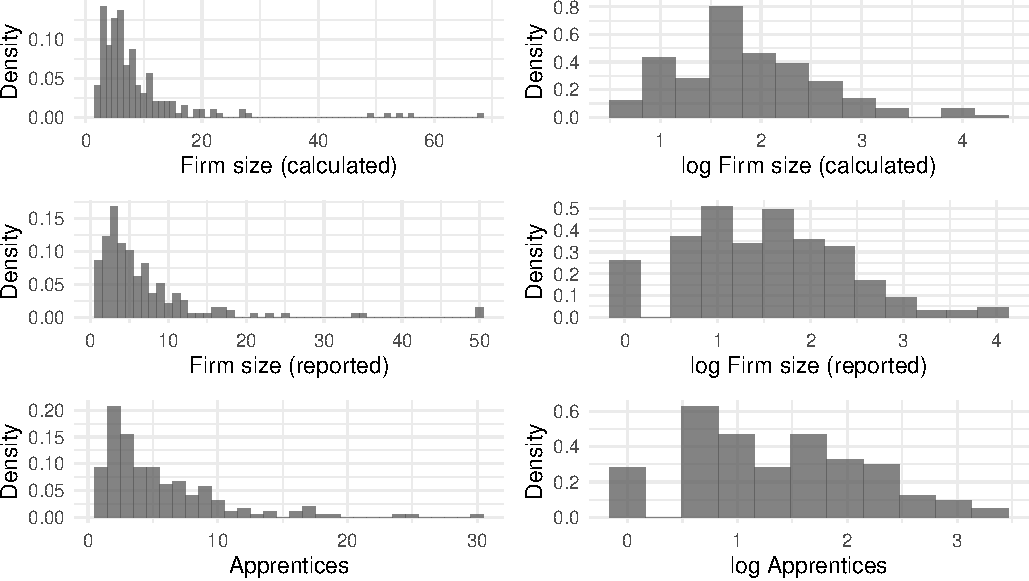
\includegraphics{figures/fig-firmsize-1} \caption{Firm size distributions}\label{fig:fig-firmsize}
\end{figure}

\begin{table}[H]

\caption{\label{tab:tbl-skillschangebycqp}Change in apprentice human capital scores}
\centering
\resizebox{\linewidth}{!}{
\begin{threeparttable}
\begin{tabular}[t]{lcccc}
\toprule
 & \textbf{CQP Selected}, N = 150 & \textbf{CQP Not Selected}, N = 112 & \textbf{Did Not Apply}, N = 172 & \textbf{p-value³}\\
\midrule
Competence¹ & 0.110 (0.201) & 0.060 (0.165) & 0.158 (0.325) & 0.12\\
Experience¹ & 0.148 (0.222) & 0.104 (0.207) & 0.206 (0.314) & 0.12\\
Competence¹ & 0.110 (0.201) & 0.060 (0.165) &  & 0.3\\
Experience¹ & 0.148 (0.222) & 0.104 (0.207) &  & 0.5\\
Knowledge² & 0.034 (0.185) & 0.017 (0.166) &  & 0.8\\
\bottomrule
\end{tabular}
\begin{tablenotes}
\item Mean (SD). Change in human capital indices between baseline and endline.
\item[1] Percent of trade-specific tasks apprentice is deemed competent in (competence) or has already successfully attempted (experience), as reported by MC. Total of 10-15 tasks, depending on trade.
\item[2] Percent of trade-specific knowledge questions answered correctly by apprentice. Total of 4 or 5 questions, depending on trade.
\item[3] Analysis of variance for three groups, Wilcoxon rank sum test for two groups
\end{tablenotes}
\end{threeparttable}}
\end{table}

\begin{table}

\caption{\label{tab:tbl-compexp2}Competence and experience, MC vs. apprentice assessment}
\centering
\resizebox{\linewidth}{!}{
\begin{threeparttable}
\begin{tabular}[t]{llccccc}
\toprule
\textbf{Group} & \textbf{Trade} & \textbf{N} & \textbf{Apprentice} & \textbf{N} & \textbf{Firm} & \textbf{p-value¹}\\
\midrule
Competence & Electrical Installation & 49 & 0.97 (0.06) & 46 & 0.98 (0.05) & 0.7\\
 & Masonry & 28 & 0.95 (0.08) & 28 & 0.94 (0.10) & >0.9\\
 & Carpentry & 14 & 0.92 (0.13) & 16 & 0.95 (0.08) & 0.5\\
 & Plumbing & 25 & 0.95 (0.13) & 22 & 0.92 (0.15) & 0.7\\
 & Metalwork & 21 & 0.90 (0.17) & 26 & 0.92 (0.15) & 0.4\\
 & CQP Selected & 79 & 0.95 (0.11) & 82 & 0.95 (0.11) & 0.6\\
 & CQP Not Selected & 58 & 0.95 (0.10) & 56 & 0.94 (0.10) & 0.9\\
\textbf{} & \textbf{Overall} & \textbf{137} & \textbf{0.95 (0.11)} & \textbf{138} & \textbf{0.95 (0.11)} & \textbf{0.6}\\
Experience & Electrical Installation & 49 & 0.97 (0.06) & 46 & 0.97 (0.06) & 0.9\\
 & Masonry & 28 & 0.95 (0.09) & 28 & 0.93 (0.11) & 0.9\\
 & Carpentry & 14 & 0.95 (0.12) & 16 & 0.99 (0.03) & 0.5\\
 & Plumbing & 25 & 0.98 (0.06) & 22 & 0.89 (0.17) & 0.019\\
 & Metalwork & 21 & 0.89 (0.16) & 26 & 0.89 (0.11) & 0.8\\
 & CQP Selected & 79 & 0.96 (0.10) & 82 & 0.93 (0.11) & 0.2\\
 & CQP Not Selected & 58 & 0.95 (0.09) & 56 & 0.94 (0.11) & >0.9\\
\textbf{} & \textbf{Overall} & \textbf{137} & \textbf{0.95 (0.10)} & \textbf{138} & \textbf{0.94 (0.11)} & \textbf{0.3}\\
\bottomrule
\end{tabular}
\begin{tablenotes}
\item Mean (SD). Proportion of trade-specific tasks apprentice is deemed competent in (competence) or has already successfully attempted (experience), as reported by MC. Total of 10-15 tasks, depending on trade. Comparison only possibly at endline as apprentices were not asked to self-assess competence and experience at baseline.
\item[1] Wilcoxon rank sum test
\end{tablenotes}
\end{threeparttable}}
\end{table}

\begin{table}[H] \centering 
  \caption{Effects of training on human capital, excluding CQP non-applicants} 
  \label{tab:tbl-appreg2} 
\small 
\begin{tabular}{@{\extracolsep{-8pt}}lcccccc} 
\\[-1.8ex]\hline 
\hline \\[-1.8ex] 
\\[-1.8ex] & \multicolumn{3}{c}{Experience} & \multicolumn{3}{c}{Competence} \\ 
\\[-1.8ex] & (1) & (2) & (3) & (4) & (5) & (6)\\ 
\hline \\[-1.8ex] 
 CQP Not Selected & $-$0.003 & $-$0.002 & 0.002 & 0.003 & 0.01 & 0.004 \\ 
  & (0.02) & (0.03) & (0.04) & (0.02) & (0.02) & (0.03) \\ 
  Endline & 0.14$^{***}$ & 0.14$^{***}$ & 0.12$^{***}$ & 0.12$^{***}$ & 0.11$^{***}$ & 0.07$^{**}$ \\ 
  & (0.02) & (0.03) & (0.03) & (0.02) & (0.03) & (0.03) \\ 
  CQP Selected x Endline &  & 0.003 & 0.03 &  & 0.02 & 0.05 \\ 
  &  & (0.04) & (0.04) &  & (0.04) & (0.03) \\ 
  Baseline experience$^1$ & 0.04$^{***}$ & 0.04$^{***}$ & 0.05$^{***}$ & 0.03$^{***}$ & 0.03$^{***}$ & 0.04$^{**}$ \\ 
  & (0.01) & (0.01) & (0.02) & (0.01) & (0.01) & (0.02) \\ 
  Firm size$^2$ & $-$0.01$^{**}$ & $-$0.01$^{**}$ & $-$0.01$^{*}$ & $-$0.002 & $-$0.002 & $-$0.0003 \\ 
  & (0.003) & (0.003) & (0.004) & (0.002) & (0.002) & (0.004) \\ 
  Total apprentices in firm & 0.004$^{**}$ & 0.004$^{**}$ & 0.03 & 0.004$^{**}$ & 0.004$^{**}$ & 0.02 \\ 
  & (0.002) & (0.002) & (0.05) & (0.002) & (0.002) & (0.05) \\ 
  Constant & 0.69$^{***}$ & 0.69$^{***}$ & 0.62 & 0.72$^{***}$ & 0.72$^{***}$ & 0.73$^{*}$ \\ 
  & (0.03) & (0.03) & (0.43) & (0.03) & (0.03) & (0.39) \\ 
 \hline \\[-1.8ex] 
Firm FE & NO & NO & YES & NO & NO & YES \\ 
Observations & 338 & 338 & 338 & 338 & 338 & 338 \\ 
R$^{2}$ & 0.19 & 0.19 & 0.75 & 0.16 & 0.16 & 0.75 \\ 
F Statistic & 15.00$^{***}$ & 13.00$^{***}$ & 2.80$^{***}$ & 13.00$^{***}$ & 11.00$^{***}$ & 2.80$^{***}$ \\ 
\hline 
\hline \\[-1.8ex] 
\textit{Note:}  & \multicolumn{6}{r}{$^{*}$p$<$0.1; $^{**}$p$<$0.05; $^{***}$p$<$0.01} \\ 
 & \multicolumn{6}{r}{Omitted category: CQP Selected.} \\ 
 & \multicolumn{6}{r}{$^1$Years of training prior to 2019.} \\ 
 & \multicolumn{6}{r}{$^2$Excluding apprentices} \\ 
\end{tabular} 
\end{table}

\begin{table}[H]

\caption{\label{tab:tbl-allowances}Monthly allowances}
\centering
\begin{threeparttable}
\resizebox{\linewidth}{!}{
\begin{tabular}[t]{llcccc}
\toprule
\textbf{Group} & \textbf{Characteristic} & \textbf{Overall}, N = 427 & \textbf{CQP Selected} & \textbf{CQP Not Selected} & \textbf{Did Not Apply}\\
\midrule
Baseline & Food & 6.66 (12.76) & 5.85 (13.54) & 8.45 (16.40) & 6.38 (10.10)\\
 & Transportation & 5.89 (18.74) & 4.67 (17.84) & 7.63 (21.45) & 5.92 (18.10)\\
 & Pocket Money & 14.68 (18.60) & 14.45 (18.62) & 16.47 (17.52) & 14.02 (19.15)\\
 & Other & 0.07 (1.06) & 0.00 (0.00) & 0.00 (0.00) & 0.14 (1.55)\\
 & Total & 27.30 (35.11) & 24.98 (37.33) & 32.55 (39.68) & 26.46 (31.20)\\
Endline & Food & 9.68 (8.04) & 7.81 (7.17) & 13.08 (7.87) & 9.17 (8.56)\\
 & Transportation & 2.91 (6.58) & 1.91 (4.24) & 3.31 (5.65) & 3.87 (9.33)\\
 & Pocket Money & 16.62 (55.33) & 18.46 (61.51) & 8.29 (16.49) & 21.49 (68.13)\\
 & Other & 0.00 (0.00) & 0.00 (0.00) & 0.00 (0.00) & 0.00 (0.00)\\
 & Total & 29.21 (54.68) & 28.18 (59.64) & 24.68 (18.43) & 34.53 (68.50)\\
Overall & Food & 7.50 (11.72) & 6.51 (11.81) & 9.98 (14.28) & 6.95 (9.84)\\
 & Transportation & 5.06 (16.35) & 3.75 (14.79) & 6.20 (17.92) & 5.50 (16.68)\\
 & Pocket Money & 15.22 (33.06) & 15.79 (38.40) & 13.78 (17.52) & 15.54 (34.97)\\
 & Other & 0.05 (0.90) & 0.00 (0.00) & 0.00 (0.00) & 0.11 (1.39)\\
 & Total & 27.83 (41.40) & 26.05 (45.76) & 29.96 (34.25) & 28.10 (41.44)\\
\bottomrule
\end{tabular}}
\begin{tablenotes}
\small
\item Mean (SD). Amounts in \$US.
\end{tablenotes}
\end{threeparttable}
\end{table}

\renewcommand{\arraystretch}{2}

\begin{table}[H]

\caption{\label{tab:tbl-allowancebounds}Allowances per apprentice per year, reported by firm}
\centering
\begin{threeparttable}
\resizebox{\linewidth}{!}{
\begin{tabular}[t]{llccc}
\toprule
Assumption & Bound & \textbf{Overall}, N = 347 & \textbf{Baseline}, N = 197 & \textbf{Endline}, N = 150\\
\midrule
\makecell[l]{12 months/year |\\ 20 days/month} & lower & 290.91 (158.68) & 284.93 (158.68) & 301.90 (158.68)\\
 & mid & 316.18 (208.26) & 304.39 (208.26) & 338.72 (208.26)\\
 & upper & 397.15 (257.85) & 384.34 (257.85) & 421.61 (257.85)\\
\makecell[l]{(F) months/year |\\ 20 days/month} & lower & 249.51 (158.68) & 238.87 (145.45) & 269.08 (158.68)\\
 & mid & 271.07 (168.60) & 256.64 (163.64) & 298.65 (197.11)\\
 & upper & 340.26 (236.36) & 324.79 (198.35) & 369.81 (257.85)\\
\makecell[l]{12 months/year |\\ 4 x (F) weeks/month} & lower & 343.66 (190.41) & 335.06 (190.41) & 359.47 (190.41)\\
 & mid & 373.36 (249.92) & 357.68 (249.92) & 403.29 (249.92)\\
 & upper & 468.69 (309.42) & 451.42 (309.42) & 501.69 (309.42)\\
\makecell[l]{(F) months/year |\\ 4 x (F) weeks/month} & lower & 297.10 (185.12) & 282.53 (174.55) & 323.87 (190.41)\\
 & mid & 322.42 (196.36) & 303.11 (180.50) & 359.30 (240.99)\\
 & upper & 404.36 (257.85) & 383.22 (226.12) & 444.73 (309.42)\\
\makecell[l]{12 months/year |\\ 4 x (A) weeks/month} & lower & 364.41 (222.15) & 337.82 (206.28) & 451.37 (222.15)\\
 & mid & 394.66 (247.60) & 360.43 (236.03) & 515.74 (291.57)\\
 & upper & 496.89 (309.42) & 455.98 (277.69) & 641.56 (360.99)\\
\makecell[l]{firm months |\\ 4 x (A) weeks/month} & lower & 317.89 (166.61) & 287.89 (166.61) & 415.98 (166.61)\\
 & mid & 344.25 (183.47) & 309.03 (180.50) & 468.83 (218.68)\\
 & upper & 432.46 (239.34) & 390.97 (206.28) & 579.15 (309.42)\\
\bottomrule
\end{tabular}}
\begin{tablenotes}
\small
\item Mean (Median). (F): reported by firm; (A): reported by apprentices. Amounts in \$US.
\end{tablenotes}
\end{threeparttable}
\end{table}

\begin{table}[H]

\caption{\label{tab:tbl-allowboundsapp}Allowances per apprentice per year, reported by apprentice}
\centering
\begin{threeparttable}
\resizebox{\linewidth}{!}{
\begin{tabular}[t]{llccc}
\toprule
Assumption & Bound & \textbf{Overall}, N = 347 & \textbf{Baseline}, N = 197 & \textbf{Endline}, N = 150\\
\midrule
\makecell[l]{12 months/year |\\ 4 weeks/month} & lower & 199.00 (198.35) & 187.81 (158.68) & 251.95 (238.02)\\
 & mid & 264.77 (238.02) & 252.64 (198.35) & 322.18 (317.36)\\
 & upper & 330.49 (277.61) & 317.41 (237.94) & 392.33 (396.61)\\
\makecell[l]{(F) months/year |\\ 4 weeks/month} & lower & 164.96 (119.01) & 153.26 (115.70) & 220.33 (218.18)\\
 & mid & 221.36 (158.68) & 208.59 (145.45) & 281.80 (290.91)\\
 & upper & 277.71 (198.27) & 263.87 (181.75) & 343.20 (363.56)\\
\bottomrule
\multicolumn{5}{l}{\rule{0pt}{1em}\textsuperscript{1} Mean (Median)}\\
\end{tabular}}
\begin{tablenotes}
\small
\item Mean (Median). (F): reported by firm; (A): reported by apprentices. Amounts in \$US.
\end{tablenotes}
\end{threeparttable}
\end{table}

\renewcommand{\arraystretch}{1}

\begin{figure}[H]
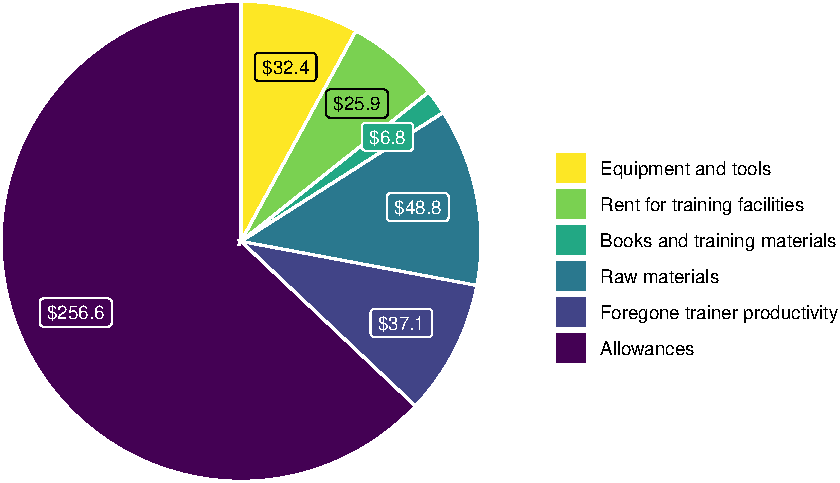
\includegraphics{figures/fig-costspie-1} \caption{Breakdown of mean annual training costs per apprentice}\label{fig:fig-costspie}
\end{figure}

\begin{figure}[H]
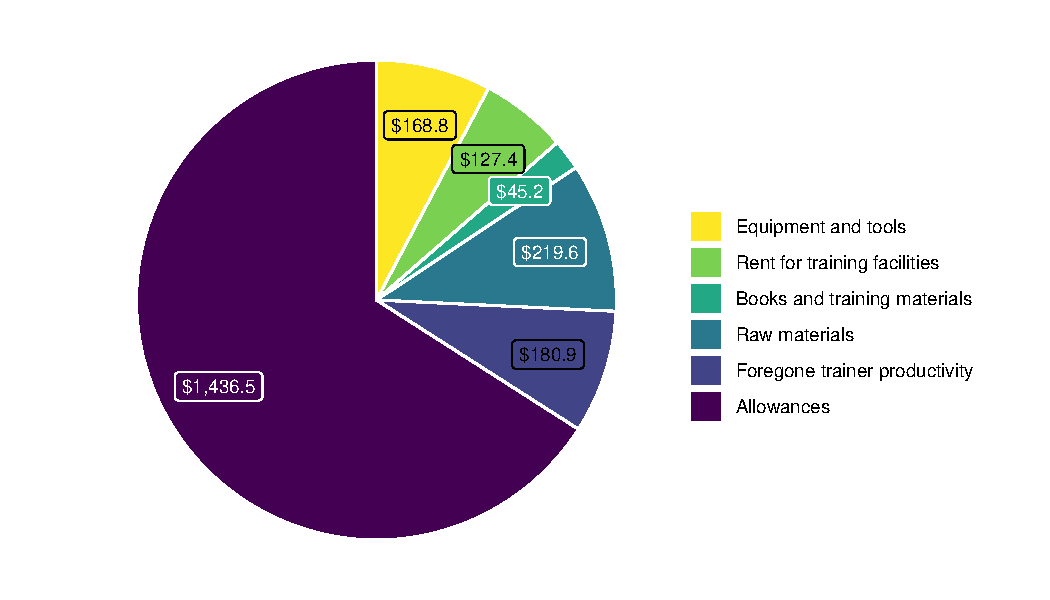
\includegraphics{figures/fig-costspie2-1} \caption{Breakdown of mean annual training costs per firm}\label{fig:fig-costspie2}
\end{figure}

\begin{table}

\caption{\label{tab:tbl-wages}Monthly wages}
\centering
\begin{tabular}[t]{lcccc}
\toprule
 & \textbf{N} & \textbf{Baseline} & \textbf{N} & \textbf{Endline}\\
\midrule
Former apprentice (diff. workshop) & 139 & 17 (56) & 140 & 17 (43)\\
Former apprentice (same workshop) & 139 & 19 (68) & 140 & 15 (43)\\
Worker with secondary educ. or more & 128 & 7 (35) & 140 & 9 (52)\\
Worker with primary educ. or less & 132 & 5 (30) & 140 & 4 (34)\\
Paid family worker & 124 & 4 (19) & 140 & 4 (18)\\
Occassional worker & 155 & 39 (77) & 145 & 27 (59)\\
Firm owner & 173 & 82 (88) & 144 & 124 (95)\\
Traditional apprentice (first year) & 172 & 0 (4) & 140 & 6 (10)\\
Traditional apprentice (third year) & 172 & 1 (6) & 140 & 11 (16)\\
CQP apprentice (first year) & 170 & 1 (6) & 140 & 3 (8)\\
CQP apprentice (third year) & 166 & 2 (9) & 140 & 13 (35)\\
\bottomrule
\multicolumn{5}{l}{\rule{0pt}{1em}\textsuperscript{1} Mean (SD). Monthly wages in \textbackslash{}\textbackslash{}\$US.}\\
\end{tabular}
\end{table}

\begin{figure}
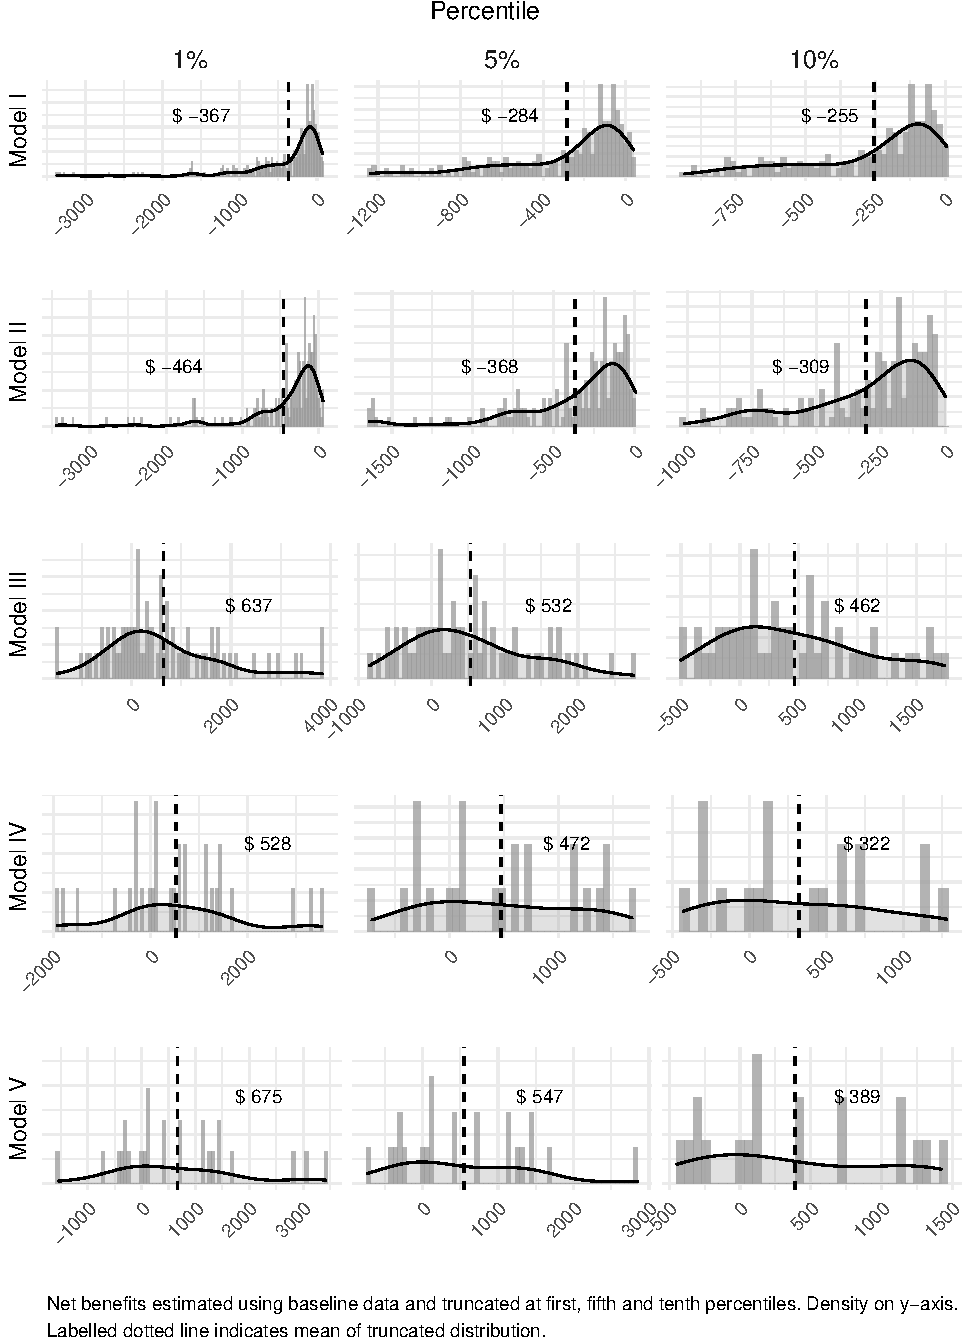
\includegraphics[width=1\linewidth,]{figures/fig-apphist-1} \caption{Distribution of net benefits per apprentice}\label{fig:fig-apphist}
\end{figure}

\begin{figure}
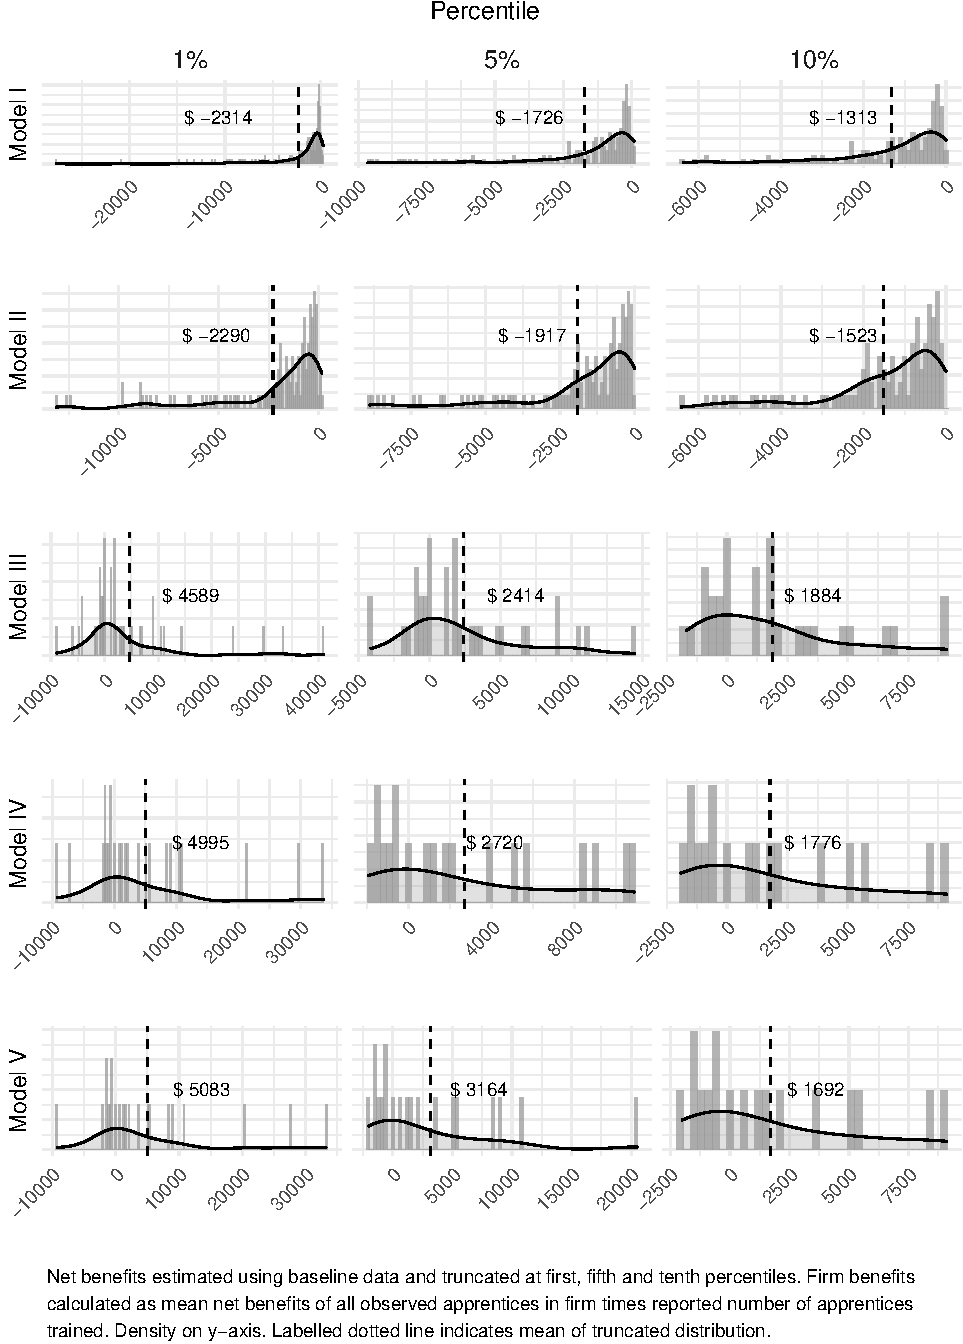
\includegraphics[width=1\linewidth,]{figures/fig-firmhist-1} \caption{Distribution of net benefits per firm}\label{fig:fig-firmhist}
\end{figure}

\begin{table}[H]

\caption{\label{tab:tbl-appnetbenefitsnodna}Annual costs and benefits per apprentice, CQP applicants only}
\centering
\resizebox{\linewidth}{!}{
\begin{threeparttable}
\begin{tabular}[t]{lccccccc}
\toprule
\textbf{Characteristic} & \textbf{N} & \textbf{Overall} & \textbf{N} & \textbf{CQP Selected} & \textbf{N} & \textbf{CQP Not Selected} & \textbf{p-value}\\
\midrule
\addlinespace[0.3em]
\multicolumn{8}{l}{\textbf{Benefits}}\\
\hspace{1em}Fees¹ & 243 & 53.60 (37.86) & 143 & 50.74 (36.67) & 100 & 57.68 (39.33) & 0.2\\
\hspace{1em}\hspace{1em}Entry & 231 & 2.53 (4.24) & 135 & 2.33 (3.30) & 96 & 2.82 (5.29) & 0.4\\
\hspace{1em}\hspace{1em}Formation & 231 & 23.82 (30.29) & 135 & 20.10 (27.58) & 96 & 29.04 (33.19) & 0.027\\
\hspace{1em}\hspace{1em}Liberation & 231 & 8.54 (18.29) & 135 & 9.44 (18.61) & 96 & 7.26 (17.86) & 0.4\\
\hspace{1em}\hspace{1em}Materials & 231 & 6.29 (9.19) & 135 & 6.35 (9.47) & 96 & 6.20 (8.83) & >0.9\\
\hspace{1em}\hspace{1em}Contract & 231 & 10.05 (18.22) & 135 & 11.01 (18.70) & 96 & 8.70 (17.52) & 0.3\\
\hspace{1em}\hspace{1em}Application & 231 & 3.05 (4.15) & 135 & 3.30 (4.25) & 96 & 2.70 (4.00) & 0.3\\
\hspace{1em}Apprentice prod. & 62 & 1,039.62 (1,172.56) & 34 & 869.20 (1,050.46) & 28 & 1,246.57 (1,294.84) & 0.2\\
\textbf{\hspace{1em}Total} & \textbf{59} & \textbf{1,099.04 (1,195.77)} & \textbf{33} & \textbf{939.01 (1,059.45)} & \textbf{26} & \textbf{1,302.16 (1,343.08)} & \textbf{0.3}\\
\addlinespace[0.3em]
\multicolumn{8}{l}{\textbf{Costs}}\\
\hspace{1em}Allowances¹ & 235 & 604.73 (1,225.89) & 135 & 583.89 (1,398.96) & 100 & 632.85 (949.56) & 0.8\\
\hspace{1em}\hspace{1em}Food & 141 & 72.79 (171.96) & 84 & 61.57 (158.26) & 57 & 89.31 (190.63) & 0.3\\
\hspace{1em}\hspace{1em}Transport & 141 & 59.73 (205.04) & 84 & 46.23 (188.52) & 57 & 79.61 (227.49) & 0.3\\
\hspace{1em}\hspace{1em}Pocket money & 141 & 150.50 (181.49) & 84 & 135.30 (169.17) & 57 & 172.89 (197.68) & 0.2\\
\hspace{1em}\hspace{1em}Other & 141 & 0.00 (0.00) & 84 & 0.00 (0.00) & 57 & 0.00 (0.00) & \\
\hspace{1em}Training costs & 147 & 126.35 (250.66) & 88 & 110.95 (251.60) & 59 & 149.32 (249.61) & 0.4\\
\hspace{1em}\hspace{1em}Rent & 147 & 30.89 (65.54) & 88 & 24.18 (52.84) & 59 & 40.90 (80.34) & 0.13\\
\hspace{1em}\hspace{1em}Equipment & 144 & 36.96 (90.62) & 88 & 24.75 (50.81) & 56 & 56.15 (129.04) & 0.042\\
\hspace{1em}\hspace{1em}Books & 143 & 9.48 (45.27) & 87 & 7.65 (40.66) & 56 & 12.32 (51.90) & 0.5\\
\hspace{1em}\hspace{1em}Raw materials & 142 & 51.79 (161.19) & 87 & 55.07 (187.93) & 55 & 46.60 (107.48) & 0.8\\
\hspace{1em}Lost trainer prod. & 141 & 34.69 (43.60) & 83 & 37.68 (47.11) & 58 & 30.40 (38.00) & 0.3\\
\textbf{\hspace{1em}Total} & \textbf{66} & \textbf{758.45 (730.85)} & \textbf{39} & \textbf{676.45 (673.07)} & \textbf{27} & \textbf{876.90 (805.36)} & \textbf{0.3}\\
\addlinespace[0.3em]
\multicolumn{8}{l}{\textbf{Net Benefits}}\\
\hspace{1em}Model I & 223 & -564.88 (1,254.43) & 130 & -547.64 (1,422.47) & 93 & -588.98 (979.25) & 0.8\\
\hspace{1em}Model II & 133 & -598.70 (725.90) & 79 & -571.18 (764.74) & 54 & -638.96 (670.01) & 0.6\\
\hspace{1em}Model III & 53 & 610.97 (1,312.97) & 29 & 444.72 (1,169.03) & 24 & 811.85 (1,468.62) & 0.3\\
\hspace{1em}Model IV & 24 & 644.01 (1,566.27) & 12 & 78.33 (1,264.37) & 12 & 1,209.68 (1,683.05) & 0.076\\
\hspace{1em}Model V & 21 & 721.95 (1,555.49) & 11 & -8.33 (1,298.95) & 10 & 1,525.25 (1,460.55) & 0.020\\
\bottomrule
\end{tabular}
\begin{tablenotes}
\small
\item Mean (SD). Amounts in \$US per apprentice per year, calculated using responses from baseline survey.
\item[1] Fees and allowances reported by firm owner. Annual fees assume apprenticeship duration of four years, annual allowances assume apprentices work 20 days a month.
\end{tablenotes}
\end{threeparttable}}
\end{table}

\begin{table}[H]

\caption{\label{tab:tbl-appnetbenefitsbywave}Annual costs and benefits per apprentice, by wave}
\centering
\resizebox{\linewidth}{!}{
\begin{threeparttable}
\begin{tabular}[t]{lccccccc}
\toprule
 & \textbf{N} & \textbf{Overall} & \textbf{N} & \textbf{Baseline} & \textbf{N} & \textbf{Endline} & \textbf{p-value}\\
\midrule
\addlinespace[0.3em]
\multicolumn{8}{l}{\textbf{Benefits}}\\
\hspace{1em}Fees¹ & 591 & 64.73 (43.35) & 403 & 65.30 (44.66) & 188 & 63.51 (40.49) & 0.9\\
\hspace{1em}\hspace{1em}Entry & 579 & 3.11 (6.23) & 391 & 2.74 (4.11) & 188 & 3.90 (9.15) & 0.2\\
\hspace{1em}\hspace{1em}Formation & 579 & 36.05 (38.19) & 391 & 35.95 (38.04) & 188 & 36.26 (38.61) & 0.6\\
\hspace{1em}\hspace{1em}Liberation & 579 & 9.19 (20.76) & 391 & 9.26 (18.70) & 188 & 9.03 (24.54) & 0.012\\
\hspace{1em}\hspace{1em}Materials & 579 & 6.07 (8.16) & 391 & 6.56 (9.31) & 188 & 5.07 (4.85) & 0.4\\
\hspace{1em}\hspace{1em}Contract & 579 & 7.30 (15.69) & 391 & 8.46 (16.92) & 188 & 4.87 (12.43) & 0.020\\
\hspace{1em}\hspace{1em}Application & 579 & 3.51 (4.18) & 391 & 3.09 (4.24) & 188 & 4.38 (3.93) & <0.001\\
\hspace{1em}Apprentice prod. & 241 & 760.05 (977.48) & 114 & 1,075.59 (1,172.98) & 127 & 476.80 (644.26) & <0.001\\
\textbf{\hspace{1em}Total} & \textbf{203} & \textbf{841.72 (996.42)} & \textbf{104} & \textbf{1,140.89 (1,198.06)} & \textbf{99} & \textbf{527.44 (585.80)} & \textbf{<0.001}\\
\addlinespace[0.3em]
\multicolumn{8}{l}{\textbf{Costs}}\\
\hspace{1em}Allowances¹ & 470 & 463.58 (955.16) & 360 & 489.37 (1,021.21) & 110 & 379.17 (693.82) & 0.023\\
\hspace{1em}\hspace{1em}Food & 368 & 77.08 (134.55) & 266 & 70.57 (147.07) & 102 & 94.05 (92.90) & <0.001\\
\hspace{1em}\hspace{1em}Transport & 368 & 52.46 (170.87) & 266 & 60.88 (195.20) & 102 & 30.51 (73.78) & >0.9\\
\hspace{1em}\hspace{1em}Pocket money & 368 & 157.37 (380.71) & 266 & 145.96 (183.74) & 102 & 187.12 (660.95) & 0.001\\
\hspace{1em}\hspace{1em}Other & 368 & 0.47 (9.05) & 266 & 0.65 (10.64) & 102 & 0.00 (0.00) & 0.5\\
\hspace{1em}Training costs & 466 & 109.15 (219.01) & 229 & 110.69 (233.24) & 237 & 107.65 (204.80) & >0.9\\
\hspace{1em}\hspace{1em}Rent & 466 & 28.54 (63.68) & 229 & 26.83 (59.79) & 237 & 30.20 (67.31) & >0.9\\
\hspace{1em}\hspace{1em}Equipment & 460 & 32.38 (75.06) & 226 & 32.61 (81.94) & 234 & 32.16 (67.92) & 0.8\\
\hspace{1em}\hspace{1em}Books & 456 & 8.80 (41.76) & 224 & 8.93 (44.17) & 232 & 8.68 (39.40) & >0.9\\
\hspace{1em}\hspace{1em}Raw materials & 454 & 41.08 (135.13) & 223 & 44.10 (140.23) & 231 & 38.16 (130.26) & >0.9\\
\hspace{1em}Lost trainer prod. & 331 & 33.60 (45.59) & 245 & 36.08 (45.78) & 86 & 26.54 (44.52) & 0.12\\
\textbf{\hspace{1em}Total} & \textbf{135} & \textbf{622.24 (647.58)} & \textbf{96} & \textbf{666.56 (698.44)} & \textbf{39} & \textbf{513.15 (492.00)} & \textbf{0.2}\\
\addlinespace[0.3em]
\multicolumn{8}{l}{\textbf{Net Benefits}}\\
\hspace{1em}Model I & 442 & -404.86 (980.27) & 341 & -437.12 (1,047.68) & 101 & -295.95 (700.14) & 0.011\\
\hspace{1em}Model II & 299 & -454.58 (679.06) & 198 & -480.28 (661.41) & 101 & -404.20 (713.08) & 0.2\\
\hspace{1em}Model III & 132 & 403.62 (1,203.22) & 75 & 726.77 (1,275.80) & 57 & -21.58 (954.96) & 0.003\\
\hspace{1em}Model IV & 88 & 121.25 (1,180.94) & 31 & 631.55 (1,406.07) & 57 & -156.28 (940.73) & 0.005\\
\hspace{1em}Model V & 54 & 295.69 (1,111.39) & 28 & 686.67 (1,378.91) & 26 & -125.38 (457.68) & 0.012\\
\bottomrule
\end{tabular}
\begin{tablenotes}
\small
\item Mean (SD). Amounts in \$US per apprentice per year, calculated using responses from baseline survey.
\item[1] Fees and allowances reported by firm owner. Annual fees assume apprenticeship duration of four years, annual allowances assume apprentices work 20 days a month.
\end{tablenotes}
\end{threeparttable}}
\end{table}

\begin{landscape}

\begin{table}[H]

\caption{\label{tab:tbl-appnetbenefitsbytrade}Annual costs and benefits per apprentice, by trade}
\centering
\resizebox{\linewidth}{!}{
\begin{threeparttable}
\begin{tabular}[t]{lccccccc}
\toprule
\multicolumn{2}{c}{ } & \multicolumn{5}{c}{\textbf{Trade}} & \multicolumn{1}{c}{ } \\
\cmidrule(l{3pt}r{3pt}){3-7}
 & \textbf{Overall} & \textbf{Masonry} & \textbf{Carpentry} & \textbf{Plumbing} & \textbf{Metalwork} & \textbf{Electrical Inst.} & \textbf{p-value}\\
\midrule
\addlinespace[0.3em]
\multicolumn{8}{l}{\textbf{Benefits}}\\
\hspace{1em}Fees¹ & 65.30 (44.66) & 70.17 (38.53) & 56.97 (42.03) & 49.98 (28.28) & 52.06 (44.50) & 78.34 (49.66) & <0.001\\
\hspace{1em}\hspace{1em}Entry & 2.74 (4.11) & 1.80 (2.65) & 1.74 (2.18) & 2.47 (3.58) & 1.05 (1.75) & 4.62 (5.45) & <0.001\\
\hspace{1em}\hspace{1em}Formation & 35.95 (38.04) & 36.74 (29.00) & 33.28 (30.91) & 21.31 (32.39) & 27.26 (33.17) & 46.84 (45.52) & <0.001\\
\hspace{1em}\hspace{1em}Liberation & 9.26 (18.70) & 15.04 (20.84) & 9.87 (17.95) & 1.99 (5.77) & 7.81 (17.74) & 9.38 (20.44) & 0.001\\
\hspace{1em}\hspace{1em}Materials & 6.56 (9.31) & 8.39 (9.26) & 5.34 (5.86) & 2.89 (3.35) & 7.16 (12.96) & 6.90 (8.88) & <0.001\\
\hspace{1em}\hspace{1em}Contract & 8.46 (16.92) & 3.68 (10.44) & 7.78 (17.15) & 19.21 (22.95) & 6.74 (14.86) & 8.24 (16.72) & 0.3\\
\hspace{1em}\hspace{1em}Application & 3.09 (4.24) & 4.62 (3.96) & 4.39 (4.09) & 2.10 (3.72) & 2.99 (3.98) & 2.28 (4.48) & <0.001\\
\hspace{1em}Apprentice prod. & 1,075.59 (1,172.98) & 1,480.90 (1,306.63) & 1,118.65 (1,328.96) & 1,666.12 (298.76) & 482.72 (382.95) & 819.63 (1,087.83) & <0.001\\
\textbf{\hspace{1em}Total} & \textbf{1,140.89 (1,198.06)} & \textbf{1,683.73 (1,396.03)} & \textbf{1,013.33 (1,182.41)} & \textbf{1,694.46 (319.67)} & \textbf{537.43 (366.98)} & \textbf{884.07 (1,110.78)} & \textbf{<0.001}\\
\addlinespace[0.3em]
\multicolumn{8}{l}{\textbf{Costs}}\\
\hspace{1em}Allowances¹ & 489.37 (1,021.21) & 502.98 (868.71) & 264.34 (237.20) & 429.50 (708.59) & 264.85 (342.57) & 749.79 (1,564.54) & <0.001\\
\hspace{1em}\hspace{1em}Food & 70.57 (147.07) & 82.21 (82.86) & 34.68 (54.89) & 38.02 (67.32) & 68.44 (79.16) & 99.56 (266.47) & <0.001\\
\hspace{1em}\hspace{1em}Transport & 60.88 (195.20) & 49.33 (84.00) & 46.62 (65.40) & 57.22 (82.98) & 4.39 (26.35) & 133.42 (369.79) & <0.001\\
\hspace{1em}\hspace{1em}Pocket money & 145.96 (183.74) & 230.00 (228.63) & 101.14 (114.89) & 80.15 (68.54) & 90.81 (147.42) & 169.81 (201.63) & <0.001\\
\hspace{1em}\hspace{1em}Other & 0.65 (10.64) & 0.00 (0.00) & 0.00 (0.00) & 0.00 (0.00) & 0.00 (0.00) & 2.71 (21.69) & 0.5\\
\hspace{1em}Training costs & 110.69 (233.24) & 139.64 (200.16) & 126.09 (339.41) & 52.95 (99.52) & 75.19 (107.92) & 137.34 (289.99) & 0.090\\
\hspace{1em}\hspace{1em}Rent & 26.83 (59.79) & 18.82 (40.33) & 3.99 (9.65) & 6.31 (26.40) & 28.76 (47.40) & 45.48 (83.14) & <0.001\\
\hspace{1em}\hspace{1em}Equipment & 32.61 (81.94) & 68.13 (140.03) & 6.60 (18.41) & 21.98 (39.25) & 11.26 (25.83) & 41.26 (86.88) & <0.001\\
\hspace{1em}\hspace{1em}Books & 8.93 (44.17) & 8.29 (25.58) & 0.35 (1.78) & 6.90 (14.26) & 0.00 (0.00) & 18.30 (71.27) & 0.006\\
\hspace{1em}\hspace{1em}Raw materials & 44.10 (140.23) & 44.40 (73.39) & 115.15 (325.67) & 17.76 (51.85) & 35.17 (78.39) & 37.61 (113.62) & 0.030\\
\hspace{1em}Lost trainer prod. & 36.08 (45.78) & 34.05 (34.14) & 62.78 (76.69) & 53.48 (59.14) & 27.94 (30.68) & 31.36 (48.34) & 0.4\\
\textbf{\hspace{1em}Total} & \textbf{666.56 (698.44)} & \textbf{648.85 (324.48)} & \textbf{479.98 (618.49)} & \textbf{551.68 (594.94)} & \textbf{337.80 (222.65)} & \textbf{1,191.18 (1,084.98)} & \textbf{<0.001}\\
\addlinespace[0.3em]
\multicolumn{8}{l}{\textbf{Net Benefits}}\\
\hspace{1em}Model I & -437.12 (1,047.68) & -450.07 (917.78) & -216.41 (251.65) & -378.49 (710.13) & -215.64 (353.20) & -682.98 (1,580.38) & 0.001\\
\hspace{1em}Model II & -480.28 (661.41) & -468.88 (294.90) & -304.93 (417.16) & -464.94 (817.96) & -263.52 (221.37) & -659.02 (849.99) & 0.019\\
\hspace{1em}Model III & 726.77 (1,275.80) & 1,186.96 (1,374.17) & 741.15 (1,073.05) & 1,424.71 (275.21) & -228.78 (682.42) & 164.80 (1,177.03) & 0.001\\
\hspace{1em}Model IV & 631.55 (1,406.07) & 822.50 (1,449.81) & 148.02 (1,560.68) & 1,273.66 (163.37) & -82.23 (291.90) & 465.08 (1,747.39) & 0.4\\
\hspace{1em}Model V & 686.67 (1,378.91) & 830.37 (1,575.09) & 122.88 (1,602.28) & 1,254.03 (141.56) & -107.30 (320.73) & 703.77 (1,563.70) & 0.6\\
\bottomrule
\end{tabular}
\begin{tablenotes}
\small
\item Mean (SD). Amounts in \$US per apprentice per year, calculated using responses from baseline survey.
\item[1] Fees and allowances reported by firm owner. Annual fees assume apprenticeship duration of four years, annual allowances assume apprentices work 20 days a month.
\end{tablenotes}
\end{threeparttable}}
\end{table}

\end{landscape}

\begin{table}[H]

\caption{\label{tab:tbl-firmnetbenefitsbywave}Annual net benefits per firm, by wave}
\centering
\resizebox{\linewidth}{!}{
\begin{threeparttable}
\begin{tabular}[t]{lccccccc}
\toprule
 & \textbf{N} & \textbf{Overall} & \textbf{N} & \textbf{Baseline} & \textbf{N} & \textbf{Endline} & \textbf{p-value}\\
\midrule
\addlinespace[0.3em]
\multicolumn{8}{l}{\textbf{Firm Accounts}}\\
\hspace{1em}Revenues & 300 & 4,405 (4,917) & 159 & 3,989 (4,820) & 141 & 4,875 (5,000) & 0.002\\
\hspace{1em}Wage bill & 344 & 1,365 (2,999) & 196 & 972 (2,352) & 148 & 1,886 (3,629) & <0.001\\
\hspace{1em}Non-wage expenses & 342 & 1,640 (3,179) & 196 & 1,593 (3,152) & 146 & 1,704 (3,224) & 0.2\\
\hspace{1em}Total expenses & 340 & 3,027 (5,183) & 195 & 2,572 (4,453) & 145 & 3,639 (5,989) & <0.001\\
\hspace{1em}Profits (reported) & 303 & 1,429 (2,159) & 167 & 1,672 (2,634) & 136 & 1,132 (1,317) & 0.029\\
\hspace{1em}Profits (calculated²) & 297 & 1,549 (3,249) & 158 & 1,701 (3,056) & 139 & 1,375 (3,459) & 0.7\\
\addlinespace[0.3em]
\multicolumn{8}{l}{\textbf{Projected benefits}}\\
\hspace{1em}Fees & 317 & 370 (451) & 189 & 347 (366) & 128 & 403 (553) & >0.9\\
\hspace{1em}Apprentice prod. & 128 & 5,655 (13,455) & 47 & 8,359 (13,033) & 81 & 4,086 (13,526) & 0.011\\
\hspace{1em}Total & 117 & 6,063 (13,708) & 46 & 8,887 (13,241) & 71 & 4,234 (13,786) & 0.011\\
\addlinespace[0.3em]
\multicolumn{8}{l}{\textbf{Projected costs}}\\
\hspace{1em}Allowances & 269 & 2,783 (6,783) & 185 & 3,207 (7,741) & 84 & 1,848 (3,803) & 0.006\\
\hspace{1em}Training costs & 292 & 497 (1,071) & 144 & 511 (1,116) & 148 & 483 (1,029) & >0.9\\
\hspace{1em}Lost trainer prod. & 169 & 199 (506) & 111 & 181 (421) & 58 & 233 (640) & 0.6\\
\hspace{1em}Total & 103 & 3,430 (4,838) & 70 & 3,190 (4,441) & 33 & 3,938 (5,628) & 0.6\\
\addlinespace[0.3em]
\multicolumn{8}{l}{\textbf{Net benefits}}\\
\hspace{1em}Model I & 258 & -2,500 (6,838) & 180 & -2,947 (7,759) & 78 & -1,469 (3,814) & 0.005\\
\hspace{1em}Model II & 206 & -2,681 (7,150) & 128 & -3,174 (8,534) & 78 & -1,870 (3,861) & 0.034\\
\hspace{1em}Model III & 86 & 2,773 (9,640) & 43 & 5,574 (12,052) & 43 & -28 (5,171) & 0.10\\
\hspace{1em}Model IV & 68 & 2,040 (9,146) & 25 & 6,431 (12,457) & 43 & -513 (5,158) & 0.034\\
\hspace{1em}Model V & 43 & 2,717 (10,714) & 23 & 6,593 (12,285) & 20 & -1,740 (6,316) & 0.013\\
\bottomrule
\end{tabular}
\begin{tablenotes}
\small
\item Mean (SD). Net benefits per firm estimated using baseline data. 
Projected costs, benefits, and net benefits calculated as mean values for all observed apprentices in 
firm times reported number of apprentices trained. Amounts in \$US.
\item[1] Firms size calculated by author as sum of all reported workers in firm, including apprentices and occasional and family workers.
\item[2] Profits recalculated by author as difference between reported revenues (first row) and reported expenses (second row).
\end{tablenotes}
\end{threeparttable}}
\end{table}

\begin{landscape}

\begin{table}[H]

\caption{\label{tab:tbl-firmnetbenefitsbytrade}Annual net benefits per firm, by trade}
\centering
\resizebox{\linewidth}{!}{
\begin{threeparttable}
\begin{tabular}[t]{lccccccc}
\toprule
\multicolumn{2}{c}{ } & \multicolumn{5}{c}{\textbf{Trade}} & \multicolumn{1}{c}{ } \\
\cmidrule(l{3pt}r{3pt}){3-7}
 & \textbf{Overall}, N = 197 & \textbf{Masonry}, N = 45 & \textbf{Carpentry}, N = 24 & \textbf{Plumbing}, N = 26 & \textbf{Metalwork}, N = 39 & \textbf{Electrical Inst.}, N = 63 & \textbf{p-value}\\
\midrule
\addlinespace[0.3em]
\multicolumn{8}{l}{\textbf{Firm Accounts}}\\
\hspace{1em}Revenues & 3,989 (4,820) & 4,924 (5,760) & 4,999 (4,256) & 2,696 (3,246) & 3,498 (4,993) & 3,477 (4,447) & 0.021\\
\hspace{1em}Wage bill & 972 (2,352) & 2,304 (4,254) & 880 (1,392) & 642 (1,182) & 277 (560) & 609 (1,147) & <0.001\\
\hspace{1em}Non-wage expenses & 1,593 (3,152) & 1,318 (2,216) & 1,415 (1,757) & 653 (828) & 1,131 (1,338) & 2,528 (4,882) & 0.016\\
\hspace{1em}Total expenses & 2,572 (4,453) & 3,622 (5,559) & 2,333 (2,835) & 1,295 (1,770) & 1,411 (1,607) & 3,138 (5,639) & 0.002\\
\hspace{1em}Profits (reported) & 1,672 (2,634) & 2,567 (4,557) & 2,243 (1,408) & 1,202 (1,428) & 1,007 (1,381) & 1,266 (1,158) & <0.001\\
\hspace{1em}Profits (calculated²) & 1,701 (3,056) & 1,243 (2,957) & 2,569 (2,369) & 1,449 (1,506) & 1,967 (4,672) & 1,662 (2,572) & 0.14\\
\addlinespace[0.3em]
\multicolumn{8}{l}{\textbf{Projected benefits}}\\
\hspace{1em}Fees & 347 (366) & 317 (256) & 212 (178) & 219 (195) & 273 (332) & 526 (485) & <0.001\\
\hspace{1em}Apprentice prod. & 8,359 (13,033) & 8,719 (11,196) & 11,109 (22,156) & 9,124 (2,244) & 4,161 (6,282) & 7,990 (13,047) & 0.4\\
\hspace{1em}Total & 8,887 (13,241) & 9,472 (11,545) & 11,347 (22,106) & 9,235 (2,157) & 4,531 (6,864) & 8,542 (13,216) & 0.4\\
\addlinespace[0.3em]
\multicolumn{8}{l}{\textbf{Projected costs}}\\
\hspace{1em}Allowances & 3,207 (7,741) & 2,529 (3,775) & 1,640 (2,966) & 4,733 (17,348) & 1,541 (2,198) & 4,865 (6,332) & <0.001\\
\hspace{1em}Training costs & 511 (1,116) & 532 (723) & 404 (564) & 215 (367) & 341 (659) & 792 (1,739) & 0.2\\
\hspace{1em}Lost trainer prod. & 181 (421) & 148 (200) & 408 (1,038) & 254 (477) & 96 (92) & 194 (435) & >0.9\\
\hspace{1em}Total & 3,190 (4,441) & 3,144 (2,226) & 1,236 (854) & 2,009 (2,835) & 1,910 (3,123) & 6,173 (7,359) & 0.005\\
\addlinespace[0.3em]
\multicolumn{8}{l}{\textbf{Net benefits}}\\
\hspace{1em}Model I & -2,947 (7,759) & -2,373 (3,872) & -1,470 (3,004) & -4,515 (17,220) & -1,245 (2,052) & -4,454 (6,299) & 0.004\\
\hspace{1em}Model II & -3,174 (8,534) & -2,748 (2,869) & -995 (910) & -5,419 (19,345) & -1,465 (2,461) & -4,325 (5,315) & <0.001\\
\hspace{1em}Model III & 5,574 (12,052) & 6,553 (9,848) & 8,494 (17,498) & 7,780 (1,858) & 291 (4,639) & 4,190 (13,916) & 0.3\\
\hspace{1em}Model IV & 6,431 (12,457) & 7,385 (11,698) & 2,772 (7,030) & 7,368 (2,441) & 767 (1,901) & 7,792 (17,945) & 0.8\\
\hspace{1em}Model V & 6,593 (12,285) & 6,835 (12,160) & 2,733 (7,067) & 7,290 (2,552) & 682 (1,909) & 9,426 (17,584) & 0.8\\
\bottomrule
\end{tabular}
\begin{tablenotes}
\small
\item Mean (SD). Net benefits per firm estimated using baseline data. 
Projected costs, benefits, and net benefits calculated as mean values for all observed apprentices in 
firm times reported number of apprentices trained. Amounts in \$US.
\item[1] Firms size calculated by author as sum of all reported workers in firm, including apprentices and occasional and family workers.
\item[2] Profits recalculated by author as difference between reported revenues (first row) and reported expenses (second row).
\end{tablenotes}
\end{threeparttable}}
\end{table}

\end{landscape}

\begin{table}[H] \centering 
  \caption{Firm-level regressions with firm fixed effects} 
  \label{tab:firmregsfe} 
\begin{tabular}{@{\extracolsep{5pt}}lcccccc} 
\\[-1.8ex]\hline 
\hline \\[-1.8ex] 
\\[-1.8ex] & \multicolumn{2}{c}{log revenues (USD)} & \multicolumn{2}{c}{log profits (USD)} & \multicolumn{2}{c}{log Firm size$^1$} \\ 
\\[-1.8ex] & (1) & (2) & (3) & (4) & (5) & (6)\\ 
\hline \\[-1.8ex] 
 Non-CQP apprentices & $-$0.01 &  & $-$0.93$^{**}$ &  & $-$0.33$^{*}$ &  \\ 
  & (0.21) &  & (0.37) &  & (0.18) &  \\ 
  CQP Selected &  & $-$0.11 &  & $-$0.94$^{**}$ &  & $-$0.33$^{**}$ \\ 
  &  & (0.18) &  & (0.38) &  & (0.16) \\ 
  Total apprentices & 0.38$^{*}$ & 0.36$^{*}$ & $-$2.10$^{***}$ & $-$2.00$^{***}$ & $-$0.20 & $-$0.30$^{*}$ \\ 
  & (0.20) & (0.19) & (0.48) & (0.48) & (0.15) & (0.15) \\ 
  Endline & 0.32 & 0.30 & $-$0.88 & $-$1.00 &  &  \\ 
  & (0.24) & (0.23) & (0.78) & (0.77) &  &  \\ 
 \hline \\[-1.8ex] 
Firm FE & YES & YES & YES & YES & YES & YES \\ 
Observations & 126 & 134 & 94 & 101 & 143 & 156 \\ 
R$^{2}$ & 0.20 & 0.24 & 0.74 & 0.69 & 0.11 & 0.14 \\ 
F Statistic & 1.90 & 2.60$^{*}$ & 6.50$^{**}$ & 6.00$^{**}$ & 2.00 & 3.20$^{*}$ \\ 
\hline 
\hline \\[-1.8ex] 
\textit{Note:}  & \multicolumn{6}{r}{$^{*}$p$<$0.1; $^{**}$p$<$0.05; $^{***}$p$<$0.01} \\ 
 & \multicolumn{6}{r}{$^1$Excluding apprentices} \\ 
\end{tabular} 
\end{table}

\hypertarget{appendix-b}{%
\section*{Appendix B}\label{appendix-b}}
\addcontentsline{toc}{section}{Appendix B}

\setcounter{figure}{0}
\renewcommand{\thefigure}{B\arabic{section}.\arabic{figure}}

\end{document}
